We are going to discuss in this chapter the ideas developed in the paper \citeonline{Byun_2023}, where asymptotics of partition functions were developed for a large class of random matrix ensembles using relatively straightforward asymptotic techniques; namely taking advantage of the orthogonal polynomials present in these models. By the end, we hope to clarify with mathematical rigor the origin for the limit-behavior expression for the \textit{Partition Function} $\pZ{N}{Q}$ given by
\begin{equation}
	\ln(\pZ{N}{Q}) = -I_Q N^2+\frac{1}{2} N\ln N+E_Q N+G\ln N+F^Q + o(1).
	\label{Equation: asymptotic for free energy}
\end{equation}

Starting from the j.d.f. of ensemble, one can often express the j.p.d.f. of the set of eigenvalues that arise from realizations of random matrices. We have seen in \autoref{Section: RMT} that these j.p.d.f. define point process - a measure on the space of configuration of eigenvalues. Partition functions perform the role of the normalization for the probability measure on j.p.d.f. of eigenvalues. In this instance, we deal with particles in the complex plane that come from \textit{random normal matrix ensembles} as defined in \autoref{Definition: polynomial ensemble}. We consider here confining potentials $Q$ that are radially symmetric as specified in \autoref{Definicao: weight-function}. For a large class of such $Q$, the first term $I_Q$ in \eqref{Equation: asymptotic for free energy} was known for a long time, given by the system's energy when distributed according to the equilibrium measure - a distribution that minimizes the system's energy. Note that this quantity was discussed in \autoref{Section: Equilibrium} when discussing the determination of the equilibrium measure. The coefficient $1/2$ of the order $N\ln N$, as well as the entropy term $E_Q$, were described in the work of \citeonline{Leble2017-yj}, also for rather large classes of $Q$. The remaining terms in this expansion appeared firstly at \citeonline{Byun_2023}. The term $G$ appears to depend only on the genus of the limiting spectrum -  whether it is an annulus or a disk  - which, surprisingly, seems to not have been observed in the previous literature.  Although some recent work, such as in \citeonline{hedenmalm2020planarorthogonalpolynomialsboundary}, may indicate a direction to expand some of these results to larger classes of potentials, the symmetry of the external potential is, so far, still a necessary condition for the techniques presented henceforth.

\section{Outline of the technique}
\label{Section: outline asymptotic}

Given some measure $\p_N (z_1, \cdots, z_N)$, one can think of its norming function. This is what is called here the partition function $\pZ{N}{}$. Its logarithm represent the free energy of the system and is a quantity of interest in physics and mathematics. To get its asymptotics we will perform the following steps.

\begin{itemize}
	\item \textit{Partition functions can be expressed in terms of the norming constants}:  Remember  \ref{Theorem: Kernel} and \eqref{Equation: univariate kernel} that stated that normal ensembles' eigenvalue univariate density can be expressed as a Kernel; a function of the orthogonal polynomial with respect to the weight function $\wf$ used to define the ensemble. An import result for normal ensembles gives the partition function as a function of the product of norming constants. Then, we can write the free energy as
	\begin{equation}
			\ln \pZ{N}{} = \ln{N!} + \sum_{j=0}^{N-1} \ln{h_j}.
	\end{equation}
	\item \textit{Asymptotics for norming constant using the asymptotic Laplace technique}: If we set the weight function as $\wf = \ee^{-NQ(z)}$ for $Q$ a radially symmetric potential, i.e. $Q(z) = q(|z|)$, the integral expression for the norming constants can be rewritten as a real line integral and approximated by the Laplace technique.
	\begin{align}
			h_j 
			& = \int_{\C} |z|^{2j} \ee^{-N Q(z)} \dd A(z), \\
			& =  \int_{\R_+} 2 r \ee^{-N \left( q(r) - \frac{2j}{N} \ln(r) \right)} \dd r, \\
			&= \int_{\R_+} 2r \ee^{-N V_{\tau(j)}(r)} \dd r \approx \ee^{-N V_{\tau(j)}(r_c(\tau(j))}.
	\end{align}
	\item \textit{Asymptotic of the summation on $h_j$ using quadrature}: Finally, to approximate the summation on $\ln(h_j)$ we use the previously discussed idea of quadrature in \autoref{section: quadrature} relating the limit summation with the corresponding integral.
	\begin{equation}
		- \sum_{j=0}^{N-1} \ln{h_j} \approx - N^2 \int_{r_0}^{r_1} V(r) \frac{(r q'(r))'}{2} \dd r = - N^2 I_Q[\mu_Q].
	\end{equation}
\end{itemize}

This technique can take us much further in order for the asymptotic expression. Above, we only used first order approximations, however in the following sections we show that doing the detailed computations, we can get all the terms down to the constant order for the asymptotic expansion. For the next section however we expand on this simplified version to give an outline for the more complex calculations. Modulo minor adaptations, the results we state for the random planar normal matrix ensemble are also valid in the context of the \textit{planar symplectic ensemble} - defined with an additional complex conjugation symmetry. We however omit this case to focus on clarity for the technique.

\subsection{An expression for the Partition Function}

We have stated a few properties of the model surrounding the potential $Q(z) = q(|z|)$. There is still a question of what are exactly the orthogonal polynomials with respect to the weight function defined. Consider $\{P_n(z) = \sum_{j=0}^{n} a_j z^j\}_{n}^{(w)}$ a family of orthogonal polynomials in respect to $w$ where $P_m$ has degree $m$. 

\begin{lema}
	The set $\{z^j\}_j^{(w)}$ is the proper orthogonal family of polynomials in relation to the weight function $w(z) = \ee^{-N Q(z)}$ defined as in as in \autoref{Definicao: weight-function}.
\end{lema}
\begin{proof}
	We know by the assumption of orthogonality that
	\begin{equation}
		\int P_n(x) P_m(x) \wf(x) \dd x = \langle P_n, P_m \rangle_w = 
		\begin{cases}
			0 & \text{if $m = n$}, \\
			1 & \text{if $m \neq n$}.
		\end{cases}
	\end{equation} 
	Let us take some arbitrary base of the polynomial space $\{z^j\}_j^{(w)}$. We apply the Gram Schmidt scheme to get the proper orthogonality in respect to the weight $w$. If $P_n = x^n$, then the orthogonal element of the basis $\tilde{P}_n$ should be
	\begin{equation}
		\tilde{P}_n = P_n - \sum_{j=0}^{n-1} \frac{\langle P_n, P_{j} \rangle_w}{\langle P_{j}, P_{j}, \rangle_w} P_{j},
	\end{equation}
	but notice that
	\begin{align}
		\langle P_n, P_{j} \rangle_w & = \int_{\C} z^{n}\bar{z}^{j} \ee^{-N Q(z)} \dd A(z), \\
		& = \int_{0}^{\infty} \int_{0}^{2\pi} r^{n-j} \ee^{\ii \theta (n - j)} \ee^{-N q(r)} r \dd r \dd \theta, \\
		& = \int_{0}^{2\pi} \ee^{\ii \theta (n - j)} \dd \theta \int_{0}^{\infty} r^{n-j+1} \ee^{-N q(r)} \dd r, \\
		& = 0, \quad \text{since} \  n \neq j.
	\end{align}
	Therefore, we have that $\{z^j\}_j^{(w)}$ is the proper orthogonal family. 
	%Moreover, if we impose normality,
	%\begin{align}
%		\int_{\C} a_n^2 z^{n-n} \ee^{-N Q(z)} \dd A(z) & = \int_{\C} a_n^2 \ee^{-N Q(z)} \dd A(z) = 1 \\
	%	& \implies a_n = \sqrt{\frac{1}{\int_{\C} w(z) \dd A(z)}}.
	%\end{align}
\end{proof}

A very important feature of the partition function of normal ensembles is that it can be expressed as a summation of norming constants of the correspondent orthogonal polynomial. This was proved on \ref{Theorem: Kernel}.
%\begin{lema}	\label{proposicaoosition: Partition function}
%	When dealing with a p.d.f. of the invariant measure given in \autoref{Definition: polynomial ensemble}, is holds that
%	\begin{equation}
%		\pZ{N}{} = N! \prod_{k=0}^{N-1} h_k,
%	\end{equation}
%	where $h_k$ is the norming constant as in $\langle q_j^{(2)}, q_k^{(2)} \rangle^{(2)} = h_j^{(2)} \chi_{j=k}$.
%\end{lema}
%\begin{proof}
%	We start stating the following equality which follows from \autoref{Theorem: Kernel} that
%	\begin{align}
%		\det\left[ K_N(\lambda_i, \lambda_j) \right]_{i,j=1}^{N} & =  p^{(w)}(\mmany{\lambda}{N}), \\
%		\prod_{k=0}^{N-1} h_k^{-1}  \det\left[ \sqrt{\wf(x) \wf(y)} \sum_{k=0}^{N-1} q_k(x) q_k(y) \right]_{i,j=1}^{N} & = \prod_{1 < i \leq j < N} (\lambda_j - \lambda_i)^2 \prod_{k=0}^{N} w(\lambda_k).
%	\end{align}
%	Therefore, rearranging the terms
%	\begin{equation}
%		N! \det\left[ \tilde{K}_N(\lambda_i, \lambda_j) \right]_{i,j=1}^{N} = N! \prod_{k=0}^{N-1} h_k \prod_{1 < i \leq j < N} (\lambda_j - \lambda_i)^2 \prod_{k=0}^{N} w(\lambda_k)
%	\end{equation}
%	where we we can check from the definition the correlation functions that
%	\begin{equation}
%		\pZ{N}{} = N! \prod_{k=0}^{N-1} h_k.
%	\end{equation}
%\end{proof}
Thus, using the expression, we write the free energy as
\begin{equation}
	\ln \pZ{N}{} = \ln{N!} + \sum_{j=0}^{N-1} \ln{h_j},  \quad \text{where} \qquad h_k \deff \int_{\C} |z|^{2j} \ee^{-N Q(z)} \dd A(z)
	\label{Equation: Partition Function}
\end{equation}
are the norming constants for the monomial family of orthogonal polynomials with respect to $\wf$ as in \eqref{Equation: Weight Function}. 


\subsection{Asymptotic on the Norming Constants}

 Now, we must study the asymptotic behavior of the norming constant described in \eqref{Equation: Partition Function}. Defining $z \deff r \ee^{\ii \theta}$ ($|z| = r$), because of the symmetry on $Q$ we write
\begin{align}
	h_j & = \int_{\Theta} \int_{\R_+} r^{2j} \ee^{-N q(r)} \frac{r}{\pi} \dd r \dd \theta, \\
	& = \frac{2 \pi}{\pi} \int_{\R_+} r^{2j+1} \ee^{-N q(r)} \dd r, \\
	& =  \int_{\R_+} 2 r \ee^{-N \left( q(r) - \frac{2j}{N} \ln(r) \right)} \dd r.
\end{align}
We redefine our potential using 
\begin{equation}
	V_{\tau(j)} = q(r) - 2 \tau(j) \ln(r),
\end{equation}
where $\tau(j) \deff j/N \in (0, 1]$. Then, rewrite the integral as
\begin{equation}
	h_j = \int_{\R_+} 2r \ee^{-N V_{\tau(j)}(r)} \dd r.
\end{equation}

Note that now $\tau$ will replace the role of the index $j$ marking the \enquote{degree} of the norming constant. Taking a look at the first derivative of the newly defined potential we find that the critical point $r_c$ must satisfy
\begin{equation}
	V'_\tau(r) = q'(r) - \frac{2\tau}{r} \quad \implies \quad r_c q'(r_c) = 2 \tau.
\end{equation}
We find a critical point of the potential $r_c$, parameterized by the degree of the polynomial we are calculating (given by $\tau$). We will denote $r_{\tau(j)}$ the $r$ such that $ r q'(r) = 2 \tau(j)$, that is, for each $\tau$ its critical point is denoted $r_{\tau(j)}$. Of course, because we know the range of $\tau$, it is worth defining the limit points when $\tau = 0$ and $\tau = 1$ as
\begin{equation}
	\begin{cases}
		r_0, \quad \text{the largest solution of} \ r q'(r) = 0, \\
		r_ 1, \quad \text{the smallest solution of} \ r q'(r) = 2.
	\end{cases}
\end{equation}
\
Note that these two radius, $r_0$ and $r_1$ define what we have called the Droplet in \autoref{Definition: Droplet}. They define the internal and external radius of the border for the equilibrium measure of the planar normal ensembles. Our main goal here is to evaluate the integral using the surroundings of the critical point. If this point is unique, then we only need to calculate the integral in a single small interval around $r_c(\tau(j)) \deff r_\tau(j)$. This is, of course, true: We mentioned that the properties on the potential directly implies that $r q'(r)$ is a strictly increasing function of $[r_0, r_1]$, then the solution must be unique. 


\begin{figure}[h!]
	\centering
	\hspace{1.1cm}
	\begin{subfigure}[t]{0.45\textwidth}
		\begin{tikzpicture}[scale=1]
			\draw[->] (0,0) -- (5,0) node[right, label] {$r$};
			\draw[->] (0,0) -- (0,3.2) node[above, label] {$rq'(r)$};
			
			\draw[thick] (-0.1,0) -- (0.1,0) node[left=4pt, label] {$0$};
			\draw[thick] (-0.1,3) -- (0.1,3) node[left=4pt, label] {$2$};
			
			\draw[thick] (1,-0.1) -- (1,0.1) node[below=5pt, label] {$r_0$};
			\draw[thick] (3,-0.1) -- (3,0.1) node[below=5pt, label] {$r_1$};
			
			% Function: zero on [0,r0], strictly increasing on [r0,r1], increasing after r1
			\draw[smooth, thick] (0,0.01) -- (1,0.01);
			\draw[smooth, thick] (1,0)
			.. controls (2.0,0.5) .. (3,2);
			\draw[smooth, thick] (3,2)
			.. controls (3.5,2.5) and (4.2,1.7) .. (4.5,3.2);
		
			\draw[thick] (-0.1,1.3) -- (0.1,1.3) node[left=4pt, label] {$2\tau$};
			\draw[gray, dashed, thin] (0,1.3) -- (3,1.3);
			
			\draw[gray, dashed, thin] (1, 0) -- (1,3);
			\draw[gray, dashed, thin] (3,0) -- (3,3);
			
			\fill (2.53,1.3) circle (1.5pt) node {};
		    \draw[gray, dashed, thin] (2.53, 0) -- (2.53,1.3);
		    \draw[thick] (2.53,-0.1) -- (2.53,0.1) node[below=5pt, label] {$r_c$};
		\end{tikzpicture}
	\end{subfigure}
	\begin{subfigure}[t]{0.45\textwidth}
		\begin{tikzpicture}[scale=1]
			\draw[->] (0,0) -- (5,0) node[right, label] {$r$};
			\draw[->] (0,0) -- (0,3.2) node[above, label] {$rq'(r)$};
			
			\draw[thick] (-0.1,0) -- (0.1,0) node[left=4pt, label] {$0$};
			\draw[thick] (-0.1,3) -- (0.1,3) node[left=4pt, label] {$2$};
			
			\draw[thick] (0,-0.1) -- (0,0.1) node[below=5pt, label] {$r_0$};
			\draw[thick] (3,-0.1) -- (3,0.1) node[below=5pt, label] {$r_1$};
			
			% Function: zero on [0,r0], strictly increasing on [r0,r1], increasing after r1
			\draw[smooth, thick] (0,0) -- (0,0);
			\draw[smooth, thick] (0,0)
			.. controls (2.0,0.9) .. (3,2);
			\draw[smooth, thick] (3,2)
			.. controls (3.5,2.8)  .. (4.5,3.3);
			
			\draw[thick] (-0.1,1.3) -- (0.1,1.3) node[left=4pt, label] {$2\tau$};
			\draw[gray, dashed, thin] (0,1.3) -- (3,1.3);
			
			\draw[gray, dashed, thin] (0, 0) -- (0,3);
			\draw[gray, dashed, thin] (3,0) -- (3,3);
			
			\fill (2.35,1.3) circle (1.5pt) node {};
			\draw[gray, dashed, thin] (2.35, 0) -- (2.35,1.3);
			\draw[thick] (2.35,-0.1) -- (2.35,0.1) node[below=5pt, label] {$r_c$};
		\end{tikzpicture}
	\end{subfigure}
	\caption{Graphs for the two cases of the function $rq'(r)$. On the left, we show the case for $r_0 > 0$, corresponding to the annulus droplet. On the right, we show the case for $r_0 = 0$, corresponding to the disk droplet.}
\end{figure}

Now, as outside the droplet the growth is not strict, the definitions of $r_0$ and $r_1$ had to be as mentioned before: Respectively the largest and smallest solution to the proper instance of $rq'(r) = 2\tau$. An important distinction must be made between the cases when $r_0 = 0$ and $r_0 > 0$, corresponding to \autoref{Subsection: Disk} and \autoref{Subsection: Annulus}, respectively.  We note that $r_\tau = r(\tau)$ defined such that $r_\tau q'(r_\tau) = 2 \tau$ is an increasing function of $\tau$ and that $r_0 \leq r_\tau \leq r_1 \ \forall \tau \in [0,2]$. Whichever the case, we show that the integral is approximated by its value on the critical point as
\begin{equation}
	h_j = \int_{\R_+} 2r \ee^{-N V_{\tau(j)}(r)} \dd r \approx \ee^{-N V_{\tau(j)}(r_c(\tau(j))}.
	\label{Equation: Asymptotic for norming constant}
\end{equation}

\subsection{Asymptotic on the Summation}

Now, we retake the expression for the free energy
\begin{equation}
	\ln \pZ{N}{} = \ln{N!} + \sum_{j=0}^{N-1} \ln{h_j}.
\end{equation}
Having the asymptotic expression \eqref{Equation: Asymptotic for norming constant} for the norming constant, we now want to estimate the summation on the logarithm of such expression. We write
\begin{equation}
	\ln \pZ{N}{} = \ln{N!} - N \sum_{j=0}^{N-1} V_{\tau(j)}(r_c(\tau(j))).
\end{equation}
Following the quadrature idea described in \autoref{section: quadrature}, we express this summation as
\begin{equation}
	N \sum_{j=0}^{N-1} V_{\tau(j)}(r_c(\tau(j)) \approx N^2 \int_{0}^{1} V_{\tau}(r_c(\tau)) \dd \tau.
\end{equation}

We remember the expression for the derivative of the potential $V'_\tau(r) = q'(r) - 2\tau/r$. Note that the critical point $r_{\tau(j)}$ satisfies $r_{\tau(j)} q'(r_{\tau(j)}) = 2 \tau(j)$. 

\begin{lema}	\label{Lema: diff r tau}
	The differential of $r$ as a function of $\tau$ is given by
	\begin{equation}
		\frac{\dd r(\tau)}{\dd \tau} = \frac{2}{r(\tau) V^{(2)}_\tau(r(\tau))} = \left. \frac{2}{(r q'(r))'} \right|_{r = r(\tau)}.
		\label{Equation: differential}
	\end{equation}
\end{lema}
\begin{proof}
	Note the differential
	\begin{equation}
		\frac{\dd r(\tau)}{\dd \tau} q'(r) + \frac{\dd r(\tau)}{\dd \tau} r q''(r) = 2
	\end{equation}
	which leads to
	\begin{align}
		\frac{\dd r(\tau)}{\dd \tau} = \frac{2}{q'(r) + rq'(r)} = \frac{2}{(r q'(r))'}.
	\end{align}
	And the result follow rearranging the terms.
\end{proof}
With \autoref{Lema: diff r tau}, we write the integral in terms of $r$ as
\begin{equation}
		N \sum_{j=0}^{N-1} V_{\tau(j)}(r_c(\tau(j)) \approx N^2 \int_{r_0}^{r_1} V(r) \frac{(r q'(r))'}{2} \dd r.
\end{equation}
This lead us to the main term in the expression  \eqref{Equation: asymptotic for free energy}, with order $N^2$. Note that this does not depend on the cases for $r_0$ bigger or equal to $0$. This difference only appears in lower order approximations. Namely, the dependency on the genus of the droplet is expressed on the coefficient of $\ln N$ order and changes from the disk  to the annulus case. This general first-term approach does not have such detail. We will, in the following section, derive the same asymptotic using very similar techniques. However, we will show that this approach is capable of capturing even constant terms if done more carefully.

\section{Asymptotics - Annulus}
\label{Subsection: Annulus}

We start by considering the annulus regime, when the droplet has $r_0 > 0$. When we say that $r_0 > 0$, we are saying that the equilibrium measure for model introduced in \autoref{Definicao: weight-function} is non-zero in the region of space equivalent to the set of points $z$ such that $|z| \in [r_0, r_1]$. Our objective with this section is to deduce the exact expression, analogous to \eqref{Equation: asymptotic for free energy}, of the asymptotic of the free energy $\ln{\pZ{N}{}}$ when $r_0 > 0$. For that, we will state the result and then follow the technique outlined in \autoref{Section: outline asymptotic}. We now state the main theorem of the section regarding the asymptotic for the partition function.%If we think of the equivalent Coulomb gas, this means the particles will concentrate in this shape when we perform an asymptotic on $N$.  This is the support for the limit measure.

\begin{figure}[h!]
	\centering
	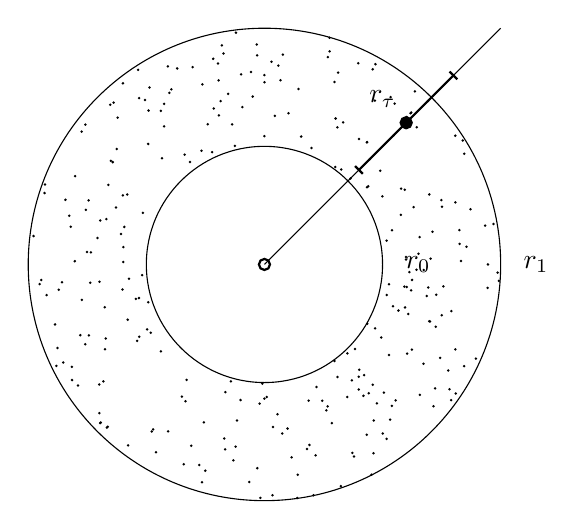
\begin{tikzpicture}[scale=1.5]
			% circles and line
			\draw (0,0) circle (1);
			\draw (0,0) circle (2);
			\draw (0,0) -- (2,2);
			\node[thick] at (0,0) {\pgfuseplotmark{o}};
			%markings fro interval
			\draw[thick] (0.8,0.8) -- (1.6,1.6);
			\node[rotate=45, thick] at (0.8,0.8) {\pgfuseplotmark{|}};
			\node[rotate=45, thick] at (1.6,1.6) {\pgfuseplotmark{|}};
			\node[thick] at (1.2,1.2) {\pgfuseplotmark{*}};
			% labels
			\node at (1.0,1.4) {$r_\tau$};
			\node at (1.3,0) {$r_0$};
			\node at (2.3,0) {$r_1$};
			% random points
			\foreach \x in {1,...,300}{
				\pgfmathsetmacro{\r}{sqrt(random(100,400)/100)}%
				\pgfmathsetmacro{\a}{random(0,360)}%
				\pgfmathsetmacro{\x}{\r*sin(\a)}
				\pgfmathsetmacro{\y}{\r*cos(\a)}
				\node[fill,circle,inner sep=0pt,minimum size=1pt] at (\x ,\y) {};
			}
	\end{tikzpicture}
	\caption{The figure depicts an annulus referring to the equilibrium measure when $r_0 > 0$. As the complex plane integral is reduced to a line integral, we draw the domain change and the point of interest $r_\tau$ where $V$ has a critical point. Around this point we depict the region around the minima, which in the method that should account for the main order of the integral we solve for.}
\end{figure}


\begin{teorema}	\label{Theorem: Annulus Free Energy}
	For the annulus case, where $r_0 > 0$, we have the following expression for the free energy asymptotically on $N$ given by
	\begin{multline}
		\ln{\pZ{N}{}} = - N^2 I_Q[\mu_Q] + \frac{N}{2} \left( \ln(2\pi) - E_Q[\mu_Q] - 2\right) + \frac{N}{2} \ln(N) \\ + \frac{\ln(2\pi)}{2} + \frac{1}{2} \ln(N)+ F_V[A_{[r_0, r_1]}] + \Boh(N^{-1})        
	\end{multline}
	where we set
	\begin{multline}
		F_V[A_{[r_0, r_1]}]  \deff - \frac{2}{3} \ln\left(\frac{r_1}{r_0} \right) + \frac{5}{32} \ln\left( \frac{V^{(2)}_1(r_1)}{V^{(2)}_0(r_0)} \right) \\ - \frac{1}{32} \left( \frac{r_1  V^{(3)}_1(r_1)}{V^{(2)}_1(r_1)} - \frac{r_0 V^{(3)}_0(r_0)}{V^{(2)}_0(r_0)}\right) - \frac{1}{12} \int_{r_0}^{r_1} \frac{V^{(3)}(r)^2}{V^{(2)}(r)^{2}} r \dd r,
	\end{multline}
	\begin{equation}
		I_Q[\mu_Q] \deff \left[\frac{1}{4} \int_{r_0}^{r_1} q(s) s V^{(2)}(s) \dd s- \ln(r_1) + \frac{1}{2} q(r_1) \right],
	\end{equation}
	and
	\begin{equation}
		E_Q[\mu_Q] \deff \frac{1}{2} \int_{r_0}^{r_1} \ln\left(\frac{V^{(2)}(s)}{4}\right) (sq'(s))' \dd s.
	\end{equation}
\end{teorema}

We start by studying the asymptotic for the norming constants $h_j$. Then, we derive the formulas for the summation on its logarithm $\ln(h_j)$. These results should be enough to prove the previous theorem. The following subsections are referring to these two results.

\subsection{Asymptotic for the norming constant}

For this subsection, we will focus on getting the asymptotic for the integral
\begin{equation}
	h_j = \int_{\R_+} 2r \ee^{-N V_{\tau(j)}(r)} \dd r
\end{equation}
for each of the degrees $j$. With this, we can proceed to examine the summation over $h_j$ needed top evaluate the free energy as it was shown in \autoref{proposicaoosition: Partition function}.


\begin{teorema}	\label{Theorem: hj annulus}
	We have the following asymptotic on $N$ for $h_j$, with $0 \leq j \leq N-1$,
	\begin{equation}
		h_j = \frac{\ee^{-N V_{\tau(j)}(r_{\tau(j)})}}{\sqrt{N}} \left( \frac{8\pi r_{\tau(j)}^2}{V^{(2)}_{\tau(j)}(r_{\tau(j)})} \right)^{\frac{1}{2}} \left[ 1 + \frac{1}{N} \mathfrak{B}(r_{\tau(j)}) + \Boh(N^{-2}) \right],
		\label{Equation: Asymptotic hj annulus}
	\end{equation}
	where we have set 
	\begin{equation}
		\mathfrak{B}(r_{\tau(j)}) \deff -\frac{V^{(4)}_{\tau(j)}(r_{\tau(j)})}{V^{(2)}_{\tau(j)}(r_{\tau(j)})^2} \frac{1}{8} - \frac{V^{(3)}_{\tau(j)}(r_{\tau(j)})}{V^{(2)}_{\tau(j)}(r_{\tau(j)})^{2}} \frac{1}{2 r_{\tau(j)}} - \frac{V^{(3)}_{\tau(j)}(r_{\tau(j)})^2}{V^{(2)}_{\tau(j)}(r_{\tau(j)})^{3}} \frac{5}{24}.
	\end{equation}
\end{teorema}

The proof for such theorem passes trough \autoref{Lema: error annulus} and \autoref{Lema: value annulus}. We begin as usual when applying asymptotic techniques in integrals; separating a central part where the integral value is concentrated and another part where we control the order of contribution. This is possible because the integrand is proportional to some exponential, with negative exponent, with a unique critical point, around which, the value of the expression concentrates, as discussed in \autoref{chapter:asymptotics}. Define $\delta_N = \ln(N)/\sqrt{N}$ - this will be the region around the critical point which contribution we will consider - then, we have
\begin{align}
	h_j =  \int_{|r - r_j| > \delta_N} 2r \ee^{-N V_{\tau(j)}(r)} \dd r + \int_{|r - r_j| < \delta_N} 2r \ee^{-N V_{\tau(j)}(r)} \dd r
	\label{Equation: Separation annulus}
\end{align}
As mentioned, the first integral must be somehow controlled and the second estimated as the main value for the result.  We begin by showing that the first term has an error contribution.

\begin{lema}	\label{Lema: error annulus}
 	We have the expression for the integral  with $|r - r_j| > \delta_N$ as in \eqref{Equation: Separation annulus} and $0 \leq j \leq N-1$, asymptotically on $N$, given by
	\begin{equation}
		\int_{|r - r_j| > \delta_N} 2r \ee^{-N V_{\tau(j)}(r)} \dd r = \ee^{-N V_{\tau(j)}(r_{\tau(j)})} \epsilon_N
	\end{equation}
	where $\epsilon_N = \Boh(\ee^{-c(\ln(N))^2})$.  
\end{lema}
\begin{proof}
	Let us first show that we can control the integral, for that, rewrite
	\begin{align}
	\int_{|r - r_j| > \delta_N} & 2r \ee^{-N V_{\tau(j)}(r)} \dd r
	\\ & = \ee^{-N V_{\tau(j)}(r_{\tau(j)})} \int_{|r - r_j| > \delta_N} 2r \ee^{-N \left( V_{\tau(j)}(r) - V_{\tau(j)}(r_{\tau(j)}) \right)} \dd r, \\
		& = \ee^{-N V_{\tau(j)}(r_{\tau(j)})} \int_{|r - r_j| > \delta_N} 2r \ee^{-N \left( V_{\tau(j)}(r) - V_{\tau(j)}(r_{\tau(j)}) \right)}  \ee^{-(M-M) \left( V_{\tau(j)}(r) - V_{\tau(j)}(r_{\tau(j)}) \right)} \dd r, \\
		& = \ee^{-N V_{\tau(j)}(r_{\tau(j)})} \int_{|r - r_j| > \delta_N} 2r \ee^{-M \left( V_{\tau(j)}(r) - V_{\tau(j)}(r_{\tau(j)}) \right)}  \ee^{-(N-M) \left( V_{\tau(j)}(r) - V_{\tau(j)}(r_{\tau(j)}) \right)} \dd r.
	\end{align}
	Now, we need some way to estimate the difference $(V_{\tau(j)}(r) - V_{\tau(j)}(r_{\tau(j)})$. If we are able to say that this difference is at least $\Boh(N^{-1})$, we control the growth of the integral choosing $M$ to be large enough such that
	\begin{equation}
		\int_{|r - r_j| > \delta_N} \left( \ee^{-q(r)} r^{2 \tau(j)} \right)^M r \dd r
	\end{equation}
	converges. Using the definition of the function $V$ and the mean value theorem, we start by evaluating the difference $\Delta(j) = V_{\tau(j+1)}(r_{\tau(j+1)}) - V_{\tau(j)}(r_{\tau(j)})$ in the following manner
	\begin{align}
		\Delta(j) &= q(r_{\tau(j+1)}) - q(r_{\tau(j)}) - 2 \left( \tau(j+1) \ln(r_{\tau(j+1)}) - \tau(j) \ln(r_{\tau(j)}) \right), \\
		& = q'(c_1) (r_{\tau(j+1)} - r_{\tau(j)}) - \frac{2}{N} \left(\ln(r_{\tau(j+1)})+j\ln\left(\frac{r_{\tau(j+1)}}{r_{\tau(j)}} \right) \right), \\
		& = q'(c_1) r'(c_2) (\tau(j+1) - \tau(j)) - \frac{2}{N} \left(\ln(r_{\tau(j+1)})+j \Boh(N^{-1}) \right), \\
		& = q'(c_1) r'(c_2) \Boh(N^{-1}) - \Boh(N^{-1}), \\
		& = \Boh(N^{-1}).
	\end{align}
	The last equality holds as both functions are continuous and $c_1, c_2$ are values that are limited; in a compact interval of the real line. Then, we add zero and use the estimation
	\begin{equation}
		V_{\tau(j+1)}(r_{\tau(j+1)})  - V_{\tau(j+1)}(r) + V_{\tau(j+1)}(r) - V_{\tau(j)}(r_{\tau(j)}) = \Boh(N^{-1})
	\end{equation}
	to derive the result we are after. It is enough to estimate $V_{\tau(j+1)}(r) - V_{\tau(j)}(r_{\tau(j)})$. For that, because $r q'(r)$ is increasing, for all $r > r_{\tau(j)} + \delta_N$ we say that
	\begin{align}
		V_{\tau(j+1)}(r) & \geq V_{\tau(j+1)}(r_{\tau(j)} + \delta_N), \\
		& =  V_{\tau(j+1)}(r_{\tau(j+1)}) + \frac{1}{2} V''_{\tau(j+1)}(r_{\tau(j+1)}) (r_{\tau(j)} + \delta_N - r_{\tau(j+1)})^2 + \Boh(\delta_N^3),
	\end{align} 
	and therefore write
	\begin{align}
		V_{\tau(j+1)}(r) - V_{\tau(j)}(r_{\tau(j)}) & =  \frac{1}{2} V''_{\tau(j+1)}(r_{\tau(j+1)}) (r_{\tau(j)} + \delta_N - r_{\tau(j+1)})^2 + \Boh(\delta_N^3), \\
		& = \delta^2 c + \Boh(N^{-1}) + \Boh(\delta_N^3), \\
		& \geq  \delta^2 c.
	\end{align}
	Finally, using the above,
	\begin{equation}
		V_{\tau(j+1)}(r) - V_{\tau(j+1)}(r_{\tau(j+1)}) \geq c \delta_N^2.
	\end{equation}

	Getting this inequality back to the integral expression end up with
	\begin{align}
		\int_{|r - r_j| > \delta_N} & 2r \ee^{-N V_{\tau(j)}(r)} \dd r \\
		& =  \ee^{-N V_{\tau(j)}(r_{\tau(j)})} \int_{|r - r_j| > \delta_N} 2r \ee^{-M \left( V_{\tau(j)}(r) - V_{\tau(j)}(r_{\tau(j)}) \right)}  \ee^{-(N-M) \left( V_{\tau(j)}(r) - V_{\tau(j)}(r_{\tau(j)}) \right)} \dd r, \\
		& \leq \ee^{-N V_{\tau(j)}(r_{\tau(j)})}  \ee^{- c \delta_N^2 (N - M)} \int_{|r - r_j| > \delta_N} 2r \ee^{-M \left( V_{\tau(j)}(r) - V_{\tau(j)}(r_{\tau(j)}) \right)} \dd r,
	\end{align}
	where one can check that
	\begin{align}
		\int_{|r - r_j| > \delta_N}  & 2r \ee^{-M \left( V_{\tau(j)}(r) - V_{\tau(j)}(r_{\tau(j)}) \right)} \dd r \\ 
		& = \int_{|r - r_j| > \delta_N} 2r \ee^{-M \left( (q(r) - 2 \tau(j) \ln(r)) - (q(r_{\tau(j)}) - 2 \tau(j) \ln(r_{\tau(j)})) \right)} \dd r,  \\
		& = 2 \left( \ee^{-q(r_{\tau(j)})} r_{\tau(j)}^{-2 \tau(j)} \right)^M \int_{|r - r_j| > \delta_N} \left( \ee^{-q(r)} r^{2 \tau(j)} \right)^M r \dd r.
	\end{align}
	By assumption, we chose $M$ to be a big enough number such that the integral above converges. If that is true, 
	\begin{equation}
		\int_{|r - r_j| > \delta_N} 2r \ee^{-N V_{\tau(j)}(r)} \dd r = \int_{|r - r_j| > \delta_N} 2r \ee^{-N V_{\tau(j)}(r)} \dd r \leq \ee^{-N V_{\tau(j)}(r_{\tau(j)})} \epsilon_N,
	\end{equation}
	with $\epsilon_N = \Boh(\ee^{-c(\ln(N))^2})$.  
\end{proof}
	
We now move on to the value-contributing part of the integral. The other order term should be absorbed in this one if \autoref{Theorem: hj annulus} is to be right.
	
\begin{lema} 	\label{Lema: value annulus}
		For the second part of the integral we have, for the integral  with $|r - r_j| > \delta_N$ as in \eqref{Equation: Separation annulus} and $0 \leq j \leq N-1$, asymptotically on $N$,
		\begin{equation}
			\int_{|r - r_j| < \delta_N} 2r \ee^{-N V_{\tau(j)}(r)} \dd r  = \frac{\ee^{-N V_{\tau(j)}(r_{\tau(j)})}}{\sqrt{N}} \left( \frac{8\pi r_{\tau(j)}^2}{V^{(2)}_{\tau(j)}(r_{\tau(j)})} \right)^{\frac{1}{2}} \left[ 1 + \frac{1}{N} \mathfrak{B}(r_{\tau(j)}) + \Boh(N^{-2}) \right]
			\label{Equation: main part annulus}
		\end{equation}
		where $\mathfrak{B}(r_{\tau(j)})$ is as in \autoref{Theorem: hj annulus}.
\end{lema}	

\begin{proof}
	As we are dealing with a symmetric (in relation to the critical point) integral, we might as well set a centralized variable $x = r - r_\tau$. With this, the integral becomes
	\begin{align}
		\int_{|r - r_j| < \delta_N} & 2r \ee^{-N V_{\tau(j)}(r)} \dd r \\
		 & = \int_{-\delta_N}^{\delta_N} 2 (x + r_{\tau(j)}) \ee^{-N V_{\tau(j)}(x + r_{\tau(j)})} \dd x, \\
		& = \ee^{-N V_{\tau(j)}(r_{\tau(j)})}  \int_{-\delta_N}^{\delta_N} 2 (x + r_{\tau(j)}) \ee^{-N \left[ V_{\tau(j)}(x + r_{\tau(j)}) - V_{\tau(j)}(r_{\tau(j)})\right]} \dd x.
	\end{align}
	Our interval grows with $\sqrt{N}/\ln(N)$. By re-scaling the reference variable using $y = \sqrt{N} x$ we get
	\begin{align}
		\int_{|r - r_j| < \delta_N} & 2r \ee^{-N V_{\tau(j)}(r)} \dd r\\ 
		&= \frac{\ee^{-N V_{\tau(j)}(r_{\tau(j)})}}{\sqrt{N}}  \int_{-\ln(N)}^{\ln(N)} 2 \left(\frac{y}{\sqrt{N}} + r_{\tau(j)} \right) \ee^{-N \left[ V_{\tau(j)}(\frac{y}{\sqrt{N}} + r_{\tau(j)}) - V_{\tau(j)}(r_{\tau(j)})\right]} \dd y.
	\end{align}
	Using Taylor expansion for $V_{\tau(j)}\left(\frac{y}{\sqrt{N}} + r_{\tau(j)}\right )$ near the critical point $r_{\tau(j)}$ to rewrite 
	\begin{align}
		& \int_{|r - r_j| < \delta_N} 2r \ee^{-N V_{\tau(j)}(r)} \dd r\\ 
		&  =\frac{\ee^{-N V_{\tau(j)}(r_{\tau(j)})}}{\sqrt{N}}  \int_{-\ln(N)}^{\ln(N)} 2 \left(\frac{y}{\sqrt{N}} + r_{\tau(j)} \right) \ee^{-N \left(\frac{y^2}{2N} V^{(2)}_{\tau(j)}(r_{\tau(j)}) + \frac{y^3}{3! N^{\frac{3}{2}}} V^{(3)}_{\tau(j)}(r_{\tau(j)}) + \frac{y^4}{4! N^2} V^{(4)}_{\tau(j)}(r_{\tau(j)})+ \Boh\left(\left(\frac{y}{\sqrt{N}}\right)^5\right) \right)} \dd y, \\
		& = \frac{\ee^{-N V_{\tau(j)}(r_{\tau(j)})}}{(2 r_{\tau(j)} )^{-1}\sqrt{N}}  \int_{-\ln(N)}^{\ln(N)} \left(\frac{y}{r_{\tau(j)}\sqrt{N}} + 1 \right) \ee^{-\frac{y^2}{2} V^{(2)}_{\tau(j)}(r_{\tau(j)}) - \frac{y^3}{3! \sqrt{N}} V^{(3)}_{\tau(j)}(r_{\tau(j)}) - \frac{y^4}{4! N} V^{(4)}_{\tau(j)}(r_{\tau(j)}) + \Boh\left(\frac{y^5}{N^\frac{3}{2}}\right)} \dd y, \\
		& = \frac{\ee^{-N V_{\tau(j)}(r_{\tau(j)})}}{(2 r_{\tau(j)} )^{-1}\sqrt{N}}  \int_{-\ln(N)}^{\ln(N)} \left(\frac{y}{r_{\tau(j)}\sqrt{N}} + 1 \right) \ee^{-\frac{y^2}{2} V^{(2)}_{\tau(j)}(r_{\tau(j)})} \left(\ee^{- \frac{y^3}{3! \sqrt{N}} V^{(3)}_{\tau(j)}(r_{\tau(j)}) - \frac{y^4}{4! N} V^{(4)}_{\tau(j)}(r_{\tau(j)}) + \Boh\left(\frac{y^5}{N^\frac{3}{2}}\right)}\right) \dd y.
	\end{align}
	Now we take the Taylor Series for 
	\begin{multline}
		\ee^{- \frac{y^3}{3! \sqrt{N}} V^{(3)}_{\tau(j)}(r_{\tau(j)}) - \frac{y^4}{4! N} V^{(4)}_{\tau(j)}(r_{\tau(j)}) + \Boh\left(\frac{y^5}{N^\frac{3}{2}}\right)} = 1 - \left[ \frac{y^3}{3! \sqrt{N}} V^{(3)}_{\tau(j)}(r_{\tau(j)}) + \frac{y^4}{4! N} V^{(4)}_{\tau(j)}(r_{\tau(j)}) + \Boh\left(\frac{y^5}{N^\frac{3}{2}}\right) \right] \\ 
		- \frac{1}{2} \left[ \frac{y^6}{N} \left(\frac{V^{(3)}_{\tau(j)}(r_{\tau(j)})}{6} \right)^2 + \frac{y^8}{N^2} \left(\frac{V^{(4)}_{\tau(j)}(r_{\tau(j)})}{24} \right)^2 + \frac{y^7}{N^3} \left(\frac{V^{(4)}_{\tau(j)}(r_{\tau(j)})}{6} \frac{V^{(3)}_{\tau(j)}(r_{\tau(j)})}{24} \right) + \Boh\left(\frac{y^8}{N^2}\right)  \right].
	\end{multline}
	To get the asymptotic expansion (since odd terms vanish) we reorganize the terms in the integral again to obtain
	\begin{multline}
		\int_{|r - r_j| < \delta_N} 2r \ee^{-N V_{\tau(j)}(r)} \dd r\\ = 2 r_{\tau(j)} \frac{\ee^{-N V_{\tau(j)}(r_{\tau(j)})}}{\sqrt{N}}  \int_{-\ln(N)}^{\ln(N)} \ee^{-\frac{y^2}{2} V^{(2)}_{\tau(j)}(r_{\tau(j)})} \left[ 1 - \frac{y^4}{3! r_{\tau(j)} N} V^{(3)}_{\tau(j)}(r_{\tau(j)}) \right. \\
		\left. - \frac{y^4}{4! N} V^{(4)}_{\tau(j)}(r_{\tau(j)}) - \frac{y^6}{2 \cdot (3!)^2 N} V^{(3)}_{\tau(j)}(r_{\tau(j)})^2 + \Boh\left(\frac{y^6}{N^2}\right) \right] \dd y,
		\label{Equation: value-contributing integral}
	\end{multline}
	then, distributing the integral,
	\begin{multline}
		\int_{|r - r_j| < \delta_N} 2r \ee^{-N V_{\tau(j)}(r)} \dd r\\ 
		 = 2 r_{\tau(j)} \frac{\ee^{-N V_{\tau(j)}(r_{\tau(j)})}}{\sqrt{N}}
		 \left[
		\left(- \frac{V^{(4)}_{\tau(j)}(r_{\tau(j)})}{24 N} - \frac{V^{(3)}_{\tau(j)}(r_{\tau(j)})}{6 r_{\tau(j)} N} \right)
		\int_{-\ln(N)}^{\ln(N)} \ee^{-\frac{y^2}{2} V^{(2)}_{\tau(j)}(r_{\tau(j)})} y^4 \dd y \right. \\
		\left. - \frac{V^{(3)}_{\tau(j)}(r_{\tau(j)})^2}{72 N}
		\int_{-\ln(N)}^{\ln(N)} \ee^{-\frac{y^2}{2} V^{(2)}_{\tau(j)}(r_{\tau(j)})} y^6 \dd y +
		\int_{-\ln(N)}^{\ln(N)} \ee^{-\frac{y^2}{2} V^{(2)}_{\tau(j)}(r_{\tau(j)})} \dd y + \Boh\left( N^{-2} \right) \right].
	\end{multline}
	At this point, the result is directly evaluated using the Gaussian integrals in \autoref{Prop: Gaussian integrals}.	So that we substitute the values to get
	\begin{multline}
		\int_{|r - r_j| < \delta_N} 2r \ee^{-N V_{\tau(j)}(r)} \dd r\\ 
		 = \sqrt{2\pi} r_{\tau(j)} \frac{\ee^{-N V_{\tau(j)}(r_{\tau(j)})}}{\sqrt{N}} \left[
		\left(- \frac{V^{(4)}_{\tau(j)}(r_{\tau(j)})}{24 N} - \frac{V^{(3)}_{\tau(j)}(r_{\tau(j)})}{6 r_{\tau(j)} N} \right) \frac{3}{16} \left( \frac{4}{V^{(2)}_{\tau(j)}(r_{\tau(j)})} \right)^{\frac{5}{2}} \right. \\
		\left. - \frac{V^{(3)}_{\tau(j)}(r_{\tau(j)})^2}{72 N} \frac{15}{64} \left(\frac{4}{V^{(2)}_{\tau(j)}(r_{\tau(j)})} \right)^{\frac{7}{2}} +
		\left( \frac{4}{V^{(2)}_{\tau(j)}(r_{\tau(j)})} \right)^{\frac{1}{2}} + \Boh\left( N^{-2} \right) \right],
	\end{multline}
	and, rearranging the terms we get our result
	\begin{equation}
		\int_{|r - r_j| < \delta_N} 2r \ee^{-N V_{\tau(j)}(r)} \dd r =  \frac{\ee^{-N V_{\tau(j)}(r_{\tau(j)})}}{\sqrt{N}} \left( \frac{8\pi r_{\tau(j)}^2}{V^{(2)}_{\tau(j)}(r_{\tau(j)})} \right)^{\frac{1}{2}} \left[ 1 + \frac{1}{N} \mathfrak{B}(r_{\tau(j)}) + \Boh(N^{-2}) \right]
		\label{Equation: main part annulus}
	\end{equation}
	where we defined $	\mathfrak{B}(r_{\tau(j)})$ as
	\begin{equation}
		\mathfrak{B}(r_{\tau(j)}) = -\frac{V^{(4)}_{\tau(j)}(r_{\tau(j)})}{V^{(2)}_{\tau(j)}(r_{\tau(j)})^2} \frac{1}{8} - \frac{V^{(3)}_{\tau(j)}(r_{\tau(j)})}{V^{(2)}_{\tau(j)}(r_{\tau(j)})^{2}} \frac{1}{2 r_{\tau(j)}} - \frac{V^{(3)}_{\tau(j)}(r_{\tau(j)})^2}{V^{(2)}_{\tau(j)}(r_{\tau(j)})^{3}} \frac{5}{24}.
	\end{equation}
	
	Notice that the error term of \autoref{Lema: error annulus} is absorbed into the error order of \eqref{Equation: main part annulus}. Therefore we have the asymptotic expression for $h_j$ given by \eqref{Equation: Asymptotic hj annulus} and the proof for \autoref{Theorem: hj annulus} follows directly.
\end{proof}

\subsection{Asymptotics on the Summation}

We return to \eqref{Equation: Partition Function} and turn to the calculation of each term of $	\sum_{j=0}^{N-1} \ln{h_j}$ using the logarithm of the expansion calculated previously in \autoref{Theorem: hj annulus}
\begin{equation}
 \sum_{j=0}^{N-1} \left[-N V_{\tau(j)}(r_{\tau(j)}) + \frac{1}{2} \left(\ln(2\pi r^2_{\tau(j)}) - \ln N - \ln\left(\frac{V^{(2)}_{\tau(j)}(r_{\tau(j)})}{4}\right)  \right) + \frac{1}{N} \mathfrak{B}(r_{\tau(j)}) + \Boh(N^{-2})\right]. 
	\label{Equation: sum log annulus}
\end{equation}

That is, we need to prove the following theorem.

\begin{teorema}			\label{Theorem: Annulus sum}
	Asymptotically on $N$,
	\begin{equation}
		\sum_{j=0}^{N-1} \ln{h_j} = - N^2 I_Q[\mu_Q] - \frac{N}{2} \ln N + N \left(\frac{\ln(2\pi)}{2} - \frac{1}{2} E_Q[\mu_Q]\right) + F_V[A_{[r_0, r_1]}] + \Boh(N^{-1}) 
	\end{equation}
	where $F_V[A_{[r_0, r_1]}]$, $I_Q[\mu_Q]$, $	E_Q[\mu_Q]$ are as in \autoref{Theorem: Annulus Free Energy}.
\end{teorema}

The proof comes from gathering the terms in \eqref{Equation: sum log annulus} with its respective expressions derived in \autoref{Lemma: Annulus sum N2} and \autoref{Lemma: Annulus Sum 1/2}. We go term by term. \autoref{Lemma: Annulus sum N2} refers to the asymptotic of 
\begin{equation}
	\sum_{j=0}^{N-1} \left(-N V_{\tau(j)}(r_{\tau(j)})\right),
\end{equation}
and \autoref{Lemma: Annulus Sum 1/2} refers to the asymptotics of both terms 
\begin{equation}
	\sum_{j=0}^{N-1}\left(\ln(2\pi r^2_{\tau(j)}) - \ln\left(\frac{V^{(2)}_{\tau(j)}(r_{\tau(j)})}{4}\right)\right).
\end{equation}
Then, the final expression appears by balancing the results.

\begin{lema} 	\label{Lemma: Annulus sum N2}
	Asymptotically on $N$,
	\begin{equation}
		- N \sum_{j=0}^{N-1} V_{\tau(j)}(r_{\tau(j)}) = - N^2 I_Q[\mu_Q] + N U_{\mu_Q}(0) - \frac{1}{6} \ln{\left( \frac{r_0}{r_1}\right)} + \Boh(N^{-2})
		\label{Equation: sum V annulus}
	\end{equation}
	where we have set $I_Q[\mu_Q]$ as in \autoref{Theorem: Annulus Free Energy} and
	\begin{equation}
		- 2 U_{\mu_Q}(0) \deff \int_{r_0}^{r_1} \ln(s) (s q'(s))' \dd s  = q(r_1) - q(r_0) + 2 \ln(r_1).
	\end{equation}
\end{lema}
	
\begin{proof}
	Using the Euler-Maclaurin formula from \autoref{Theorem: Euler-Maclaurin}, 
	\begin{multline}
		\sum_{j=0}^{N-1} V_{\tau(j)}(r_{\tau(j)}) = \int_0^N V_{\tau(t)}(r_{\tau(t)})  \dd t - \frac{1}{2} \left( V_{\tau(N)}(r_{\tau(N)})  - V_{\tau(0)}(r_{\tau(0)}) \right) + \\ \frac{1}{12} \left[ \partial_t V_{\tau(t)}(r_{\tau(t)}) |_{t=N} - \partial_t V_{\tau(t)}(r_{\tau(t)}) |_{t=0} \right] + \Boh(N^{-3}).
		\label{Equation: EulerMaclaurin 1 annulus}
	\end{multline}
	The first term in \eqref{Equation: EulerMaclaurin 1 annulus} is solved doing a integral by parts. Setting $s = r_{\tau(t)}$,
	\begin{align}
		\int_0^N V_{\tau(t)}(r_{\tau(t)})  \dd t & = \int_0^N (q(r_{\tau(t)}) - 2 \tau(t) \ln(r_{\tau(t)})) \dd t, \\
		& = \frac{1}{2} \int_{r_0}^{r_1} (q(s) - s q'(s) \ln(s)) s V^{(2)}(s) N \dd s, \\
		& = N \left[  \frac{1}{2} \int_{r_0}^{r_1} q(s) s V^{(2)}(s) \dd s -  \frac{1}{2} \int_{r_0}^{r_1} s^2 q'(s) \ln(s) V^{(2)}(s) \dd s \right],
	\end{align}
	and finally using that $r_1 q'(r_1) = 2$ and $r_0 q'(r_0) = 0$ we apply the integration by parts on the second term to get
	\begin{align}
		\frac{1}{2} \int_{r_0}^{r_1} s^2 q'(s) \ln(s) V^{(2)}(s) \dd s & = \frac{1}{2} \int_{r_0}^{r_1} s^2 q'(s) \ln(s) \frac{1}{s} (s q'(s))' \dd s, \\
		&= \frac{1}{2} \int_{r_0}^{r_1} s q'(s) \ln(s) (s q'(s))' \dd s, \\
		& = \frac{1}{4} \int_{r_0}^{r_1} ((sq'(s))^2)' \ln(s) \dd s, \\
		& = \frac{1}{4} (s q'(s))^2 \ln(s) \Big|_{r_0}^{r_1} - \frac{1}{4}  \int_{r_0}^{r_1} (s q'(s))^2 \frac{1}{s} \dd s \\
		& = \ln(r_1) - \frac{1}{4} \int_{r_0}^{r_1} s q'(s)^2 \dd s, \\
		& = \ln(r_1) - \frac{1}{2} q(r_1) + \frac{1}{4} \int_{r_0}^{r_1} q(s) (s q'(s))' \dd s.
	\end{align}
	Leaving us with, by definition of $I_Q$
	\begin{align}
		\int_0^N V_{\tau(t)}(r_{\tau(t)})  \dd t & = N \left[\frac{1}{2} \int_{r_0}^{r_1} q(s) s V^{(2)}(s) \dd s - \ln(r_1) + \frac{1}{2} q(r_1) - \frac{1}{4} \int_{r_0}^{r_1} q(s) (s q'(s))' \dd s \right],  \\
		& = N \left[\frac{1}{4} \int_{r_0}^{r_1} q(s) s V^{(2)}(s) \dd s- \ln(r_1) + \frac{1}{2} q(r_1) \right],  \\
		& \revdeff N I_Q[\mu_Q].
		\label{Equation: Equilibrium energy annulus}
	\end{align}
	We also need an expression for $ V_{\tau(j)}(r_{\tau(j)})  - V_{\tau(0)}(r_{\tau(0)})$. This is direct noting that
	\begin{equation}
		V_{\tau(j)}(r_{\tau(j)})  - V_{\tau(0)}(r_{\tau(0)}) = V_1(r_1) - V_0(r_0) = q(r_1) - q(r_0) + 2 \ln(r_1) \revdeff 2 U_{\mu_Q}(0).
		\label{Equation: U function annulus}
	\end{equation}
	And finally for the remaining term we use the Leibniz rule to obtain
	\begin{align}
		\partial_t V_{\tau(t)}(r_{\tau(t)})|_{t=N}	& = \partial_t \left( q(r_{\tau(t)}) - 2 \tau(t) \ln(r_{\tau(t)}) \right)_{t=N}, \\
		& = \partial_\tau \left( q(r_{\tau(t)}) - 2 \tau(t) \ln(r_{\tau(t)}) \right)_{\tau=1} \partial_t \left( \tau(t) \right)_{t =N}, \\
		& = \frac{1}{N} \left( \partial_\tau (q(r_{\tau})) - 2 \left( \ln(r_{\tau}) + \tau \partial_\tau\left( \ln(r_{\tau}) \right)_{\tau = 1} \right) \right), \\
		& = \frac{1}{N} \left[ \partial_t(q(r_{\tau(t)}) - 2 \ln(r_{\tau(t)}))_{\tau=1} - 2 \ln(r_1) \right]
	\end{align}
	and
	\begin{equation}
		\partial_t V_{\tau(t)}(r_{\tau(t)})|_{t=0} = \frac{1}{N} \left[ \partial_t(q(r_{\tau(t)}) - 2 \ln(r_{\tau(t)}))_{\tau= 0} - 2 \ln(r_0) \right].
	\end{equation}
	Since we can calculate, from $r_1 q'(r_1) = 2$ and $r_0 q'(r_0) = 0$
	\begin{equation}
		\partial_\tau q(r_{\tau}) |_{\tau = 0} = \left( \frac{2 q'(r)}{(r q'(r))'}\right)_{r_0} = 0,
	\end{equation}
	\begin{equation}
		\partial_\tau q(r_{\tau}) |_{\tau = 1} = \left( \frac{2 q'(r)}{(r q'(r))'}\right)_{r_1} = \frac{4}{r_1(q'(r_1) + r_1 q''(r_1))},
	\end{equation}
	\begin{equation}
		\partial_\tau (2 \ln(r_\tau)) |_{\tau = 1} = \left( \frac{4}{r (r q'(r))'}\right)_{r_1} = \frac{4}{r_1(q'(r_1) + r_1 q''(r_1))},
	\end{equation}
	we also express the difference as
	\begin{equation}
		\partial_t V_{\tau(t)}(r_{\tau(t)})|_{t=N}  - \partial_t V_{\tau(t)}(r_{\tau(t)})|_{t=0} = \frac{1}{12 N} \left[ 2 (\ln(r_0) - \ln(r_1)) \right] = \frac{1}{6 N} \ln\left(\frac{r_0}{r_1}\right) .
		\label{Equation: log annulus}
	\end{equation}
	The proof for the summation $\sum_{j=0}^{N-1} V_{\tau(j)}(r_{\tau(j)})$ is complete if one gathers the terms in \eqref{Equation: Equilibrium energy annulus}, \eqref{Equation: log annulus} and \eqref{Equation: U function annulus},

\end{proof}

\begin{lema}	\label{Lemma: Annulus Sum 1/2}
		Asymptotically on $N$,
		\begin{equation}
		\sum_{j=0}^{N-1}  \ln V^{(2)}_{\tau(j)}(r_{\tau(j)})  = N E_Q[\mu_Q] -   \frac{1}{2} \ln \left( \frac{V^{(2)}_{1}(r_1)}{V^{(2)}_{0}(r_{0})} \right) + \Boh(N^{-1})
		\label{Equation: logV annulus}
	\end{equation}
	and
	\begin{equation}
		\sum_{j=0}^{N-1}  \ln(2\pi r^2_{\tau(j)}) = N \ln(2\pi) + 2 \left( - N U_{\mu_Q}(0) - \frac{1}{2} \ln\left(\frac{r_1}{r_0}\right) + \Boh(N^{-1}) \right) 
		\label{Equation: log(r) annulus}
	\end{equation}
	where $U_{\mu_Q}(0)$ as in \autoref{Lemma: Annulus sum N2} and $	E_Q[\mu_Q]$ as in \autoref{Theorem: Annulus Free Energy}.
\end{lema}

\begin{proof}
	Lets start now with the second summation, to which we apply Euler-Maclaurin again
	\begin{multline}
		\sum_{j=0}^{N-1} \ln\left(\frac{V^{(2)}_{\tau(j)}(r_{\tau(j)})}{4}\right) = \int_{0}^{N} \frac{1}{4} \ln V^{(2)}_{\tau(t)}(r_{\tau(t)}) \dd t - \frac{1}{2} \ln \left( \frac{V^{(2)}_{1}(r_1)}{V^{(2)}_{0}(r_{0})} \right) + \\ \frac{1}{12} \left[ \partial_t \frac{1}{4} \ln V^{(2)}_{\tau(t)}(r_{\tau(t)}) |_{t=N} - \partial_t \frac{1}{4} \ln V^{(2)}_{\tau(t)}(r_{\tau(t)}) |_{t=0}\right]  + \Boh(N^{-3}).
	\end{multline}
	We first tackle the integral on the right hand side, changing variables as $s = r_{\tau(t)}$ we have
	\begin{equation}
		\int_{0}^{N} \ln \frac{1}{4} V^{(2)}_{\tau(t)}(r_{\tau(t)}) \dd t = \frac{N}{2} \int_{r_0}^{r_1} \ln\left( \frac{1}{4} V^{(2)}(s)\right) (sq'(s))' \dd s.
	\end{equation}
	And, noticing that
	\begin{equation}
		\partial_t \frac{1}{4} \ln V^{(2)}_{\tau(t)}(r_{\tau(t)}) = \partial_V \left( \ln \frac{1}{4} V^{(2)}_{\tau(t)}(r_{\tau(t)}) \right) \frac{1}{4} \partial_r \left( V^{(2)}_{\tau(t)}(r_{\tau(t)}) \right) \partial_\tau \left( r_{\tau(t)} \right) = \frac{\left(\partial_r V^{(2)}\right)(r_{\tau(t)})}{r_{\tau(t)} \left( V^{(2)}_{\tau(t)}(r_{\tau(t)})\right)^2},
	\end{equation}
	we have for the third term on the right hand side, 
	\begin{align}
		\partial_t \ln \frac{1}{4} V^{(2)}_{\tau(t)}(r_{\tau(t)}) |_{t=N} - \partial_t \ln \frac{1}{4} V^{(2)}_{\tau(t)}(r_{\tau(t)}) |_{t=0} & = \frac{1}{2N} \left( \frac{\left(\partial_r V^{(2)}\right)(r_{1})}{r_1 \left( V^{(2)}_1(r_1)\right)^2} - \frac{\left(\partial_r V^{(2)}\right)(r_{0})}{r_0 \left( V^{(2)}_0(r_0)\right)^2}\right) \\ & = \Boh(N^{-1}).
	\end{align}
	Therefore,
	\begin{align}
		\sum_{j=0}^{N-1}  \ln \frac{1}{4} V^{(2)}_{\tau(j)}(r_{\tau(j)})  & = \frac{N}{2} \int_{r_0}^{r_1} \ln\left(\frac{1}{4} V^{(2)}(s)\right) (sq'(s))' \dd s  -   \frac{1}{2} \ln \left( \frac{V^{(2)}_{1}(r_1)}{V^{(2)}_{0}(r_{0})} \right) + \Boh(N^{-1}), \\
		& \deff N E_Q[\mu_Q]  -   \frac{1}{2} \ln \left( \frac{V^{(2)}_{1}(r_1)}{V^{(2)}_{0}(r_{0})} \right) + \Boh(N^{-1}).		
		\label{Equation: logV annulus}
	\end{align}
	
	Similarly, for the first summation, we apply Euler-Maclaurin again
	\begin{multline}
		\sum_{j=0}^{N-1}  \ln(2 \pi r^2_{\tau(j)}) = \ln(2\pi) + 2 \left( \int_{0}^{N} \ln(r_{\tau(t)})  \dd t - \frac{1}{2} \ln\left(\frac{r_1}{r_0}\right) \right. \\ \left. + \frac{1}{12} \left[ \partial_t \ln r_{\tau(t)} |_{\tau=1} - \partial_t \ln r_{\tau(t)} |_{\tau=0}\right] + \Boh(N^{-3}) \right).
	\end{multline}
	We first tackle the integral on the right hand side, changing variables as $s = r_{\tau(t)}$ we have
	\begin{equation}
		\int_{0}^{N} \ln r_{\tau(t)} \dd t = \frac{N}{2} \int_{r_0}^{r_1} \ln(s) (s q'(s))' \dd s.
	\end{equation}
	And, noticing that
	\begin{equation}
		\partial_t \ln r_{\tau(t)} =  \partial_r \left( \ln(r_{\tau(t)}) \right) \partial_\tau \left( r_{\tau(t)} \right) = \frac{2}{V^{(2)}_{\tau(t)}(r_{\tau(t)}) \left( r_{\tau(t)} \right)^2},
	\end{equation}
	we have for the third term on the right hand side, 
	\begin{align}
		\partial_t \ln  r_{\tau(t)} |_{\tau=1} - \partial_t \ln  r_{\tau(t)}  |_{\tau=0}  = \frac{1}{2N} \left( \frac{2}{V^{(2)}(r_{1}) \left( r_{1} \right)^2} - \frac{2}{V^{(2)}(r_{0}) \left( r_{0} \right)^2} \right) = \Boh(N^{-1}).
	\end{align}
	Then
	\begin{equation}
		\sum_{j=0}^{N-1}  \ln(2\pi r^2_{\tau(j)}) = N \ln(2\pi) + 2 \left( \frac{N}{2} \int_{r_0}^{r_1} \ln(s) (s q'(s))' \dd s - \frac{1}{2} \ln\left(\frac{r_1}{r_0}\right) + \Boh(N^{-1}) \right) .
		\label{Equation: log(r) annulus}
	\end{equation}
\end{proof}

For the following proof, and the analogous proof for the following section, we use the auxiliary result on Gaussian integrals.


\begin{proposicao}	\label{Prop: Gaussian integrals}
	The Gaussian integrals below are evaluated as follows.
	\begin{equation}
		\int_{\R} \ee^{-2ar^2} \dd r = \sqrt{\frac{\pi}{2}} \frac{1}{a^{1/2}}, \quad 	\int_{\R} \ee^{-2ar^2} r^4 \dd r = \sqrt{\frac{\pi}{2}} \frac{3}{16} \frac{1}{a^{5/2}} \quad \text{and} \quad \int_{\R} \ee^{-2ar^2} r^6 \dd r = \sqrt{\frac{\pi}{2}} \frac{15}{64} \frac{1}{a^{7/2}}.
	\end{equation}
	Moreover,
	\begin{equation}
		\quad \int_{\R} \ee^{- 2 \left( \frac{V^{(2)}_{\tau(j)}(r_{\tau(j)})}{4} \right) y^2} = \sqrt{\frac{\pi}{2}} \left( \frac{4}{V^{(2)}_{\tau(j)}(r_{\tau(j)})} \right)^{\frac{1}{2}},
	\end{equation}
	\begin{equation}
		\quad \int_{\R} \ee^{- 2 \left( \frac{V^{(2)}_{\tau(j)}(r_{\tau(j)})}{4} \right) y^2} y^4 = \sqrt{\frac{\pi}{2}} \frac{3}{16} \left(\frac{4}{V^{(2)}_{\tau(j)}(r_{\tau(j)})} \right)^{\frac{5}{2}},
	\end{equation}
	\begin{equation}
		\quad \int_{\R}\ee^{- 2 \left( \frac{V^{(2)}_{\tau(j)}(r_{\tau(j)})}{4} \right) y^2} y^6 = \sqrt{\frac{\pi}{2}} \frac{15}{64} \left( \frac{4}{V^{(2)}_{\tau(j)}(r_{\tau(j)})} \right)^{\frac{7}{2}}.
	\end{equation}
\end{proposicao}

We now move on to the proof of \autoref{Theorem: Annulus sum}.

\begin{proof} (\autoref{Theorem: Annulus sum})
	We only need to notice now that by \autoref{Theorem: Euler-Maclaurin}
	\begin{align}
		\frac{1}{N} \sum_{j=0}^{N-1} \mathfrak{B}(r_{\tau(j)}) & = \frac{1}{4} \int_{0}^{r_1} \mathfrak{B}(s) (s q'(s))' \dd s + \Boh(N^{-2}), \\
		& = \frac{1}{4} \int_{0}^{r_1} \mathfrak{B}(s) s V^{(2)}(s) \dd s + \Boh(N^{-2}).
	\end{align}
	Using the definition for $\mathfrak{B}(r_{\tau(j)})$ and integrating by parts,
	\begin{align}
		\frac{1}{N} \sum_{j=0}^{N-1} & \mathfrak{B}(r_{\tau(j)}) = \\
		& \frac{1}{4} \int_{r_0}^{r_1} \left[ -\frac{V^{(4)}(r)}{V^{(2)}(r)^2} \frac{1}{8} - \frac{V^{(3)}(r)}{V^{(2)}(r)^{2}} \frac{1}{2 r} - \frac{V^{(3)}(r)^2}{V^{(2)}(r)^{3}} \frac{5}{24} \right] r V^{(2)}(r) \dd r + \Boh(N^{-2}),\\
		& = - \frac{1}{32} \int_{r_0}^{r_1} \frac{V^{(4)}(r)}{V^{(2)}(r)} r \dd r - \frac{1}{8} \int_{r_0}^{r_1} \frac{V^{(3)}(r)}{V^{(2)}(r)} \dd r - \frac{5}{96} \int_{r_0}^{r_1} \frac{V^{(3)}(r)^2}{V^{(2)}(r)^{2}} r \dd r + \Boh(N^{-2}),\\
		& = - \frac{1}{8} \ln\left( \frac{V^{(2)}_1(r_1)}{V^{(2)}_0(r_0)} \right) - \frac{1}{32} \int_{r_0}^{r_1} \frac{V^{(4)}(r)}{V^{(2)}(r)} r \dd r - \frac{5}{96} \int_{r_0}^{r_1} \frac{V^{(3)}(r)^2}{V^{(2)}(r)^{2}} r \dd r + \Boh(N^{-2}),
	\end{align}
	where
	\begin{equation}
		 \int_{r_0}^{r_1} \frac{V^{(4)}(r)}{V^{(2)}(r)} r \dd r =  \frac{r_1  V^{(3)}_1(r_1)}{V^{(2)}_1(r_1)} - \frac{r_0 V^{(3)}_0(r_0)}{V^{(2)}_0(r_0)} - \ln \left( \frac{V^{(2)}_1(r_1)}{V^{(2)}_0(r_0)}\right) +   \int_{r_0}^{r_1} \frac{V^{(3)}(r)^2}{V^{(2)}(r)^{2}} r \dd r.
	\end{equation}
	Therefore
	\begin{multline}
			\frac{1}{N} \sum_{j=0}^{N-1} \mathfrak{B}(r_{\tau(j)})  \\ = - \frac{3}{32} \ln\left( \frac{V^{(2)}_1(r_1)}{V^{(2)}_0(r_0)} \right) - \frac{1}{32} \left( \frac{r_1  V^{(3)}_1(r_1)}{V^{(2)}_1(r_1)} - \frac{r_0 V^{(3)}_0(r_0)}{V^{(2)}_0(r_0)}\right) - \frac{1}{12} \int_{r_0}^{r_1} \frac{V^{(3)}(r)^2}{V^{(2)}(r)^{2}} r \dd r + \Boh(N^{-2}),
			\label{Equation: Summation on B}
	\end{multline}
	and the theorem follows from
	\begin{multline}
			\sum_{j=0}^{N-1} \ln{h_j} = - N^2 I_Q[\mu_Q] + N U_{\mu_Q}(0) - \frac{1}{6} \ln{\left( \frac{r_0}{r_1}\right)}  - \frac{N}{2} \ln(N) - \frac{1}{2}  \left( N E_Q[\mu_Q] -  \frac{1}{2} \ln \left( \frac{V^{(2)}_{1}(r_1)}{V^{(2)}_{0}(r_{0})} \right) \right)	\\ + \frac{1}{2} \left( N \ln(2\pi) + 2 \left( - N U_{\mu_Q}(0) - \frac{1}{2} \ln\left(\frac{r_1}{r_0}\right) \right) \right)
		 	- \frac{3}{32} \ln\left( \frac{V^{(2)}_1(r_1)}{V^{(2)}_0(r_0)} \right) \\ - \frac{1}{32} \left( \frac{r_1  V^{(3)}_1(r_1)}{V^{(2)}_1(r_1)} - \frac{r_0 V^{(3)}_0(r_0)}{V^{(2)}_0(r_0)}\right) - \frac{1}{12} \int_{r_0}^{r_1} \frac{V^{(3)}(r)^2}{V^{(2)}(r)^{2}} r \dd r +  \Boh(N^{-1})
	\end{multline}
	that reduces to
	\begin{multline}
		\sum_{j=0}^{N-1} \ln{h_j} = - N^2 I_Q[\mu_Q] - \frac{N}{2} \ln(N) + N \left(\frac{\ln(2\pi)}{2} - \frac{1}{2} E_Q[\mu_Q]\right) - \frac{2}{3}  \ln{\left( \frac{r_0}{r_1}\right)}  + \frac{5}{32} \ln \left( \frac{V^{(2)}_{1}(r_1)}{V^{(2)}_{0}(r_{0})} \right) \\ - \frac{1}{32} \left( \frac{r_1  V^{(3)}_1(r_1)}{V^{(2)}_1(r_1)} - \frac{r_0 V^{(3)}_0(r_0)}{V^{(2)}_0(r_0)}\right) - \frac{1}{12} \int_{r_0}^{r_1} \frac{V^{(3)}(r)^2}{V^{(2)}(r)^{2}} r \dd r +  \Boh(N^{-1}).
	\end{multline}
\end{proof}

%\subsubsection{Free Energy Annulus}

\begin{proof} (\autoref{Theorem: Annulus Free Energy})
	From \autoref{Theorem: hj annulus},
	\begin{multline}
		\sum_{j=0}^{N-1} \ln(h_j) = - N^2 I_Q[\mu_Q] - \frac{N}{2} \ln(N) + N \left(\frac{\ln(2\pi)}{2} - \frac{1}{2} E_Q[\mu_Q]\right) - \frac{2}{3}  \ln{\left( \frac{r_0}{r_1}\right)} +\frac{5}{32} \ln \left( \frac{V^{(2)}_{1}(r_1)}{V^{(2)}_{0}(r_{0})} \right) \\ - \frac{1}{32} \left( \frac{r_1  V^{(3)}_1(r_1)}{V^{(2)}_1(r_1)} - \frac{r_0 V^{(3)}_0(r_0)}{V^{(2)}_0(r_0)}\right) - \frac{1}{12} \int_{r_0}^{r_1} \frac{V^{(3)}(r)^2}{V^{(2)}(r)^{2}} r \dd r +  \Boh(N^{-1}).  
	\end{multline}
	We get the asymptotic expansion for the Free energy using that
	\begin{equation}
		\ln(N!) = N\ln(N) - N + \frac{1}{2} \ln(N) + \frac{1}{2} \ln(2 \pi) + \Boh(N^{-1})
	\end{equation}
	that is,
	\begin{align}
		& \ln \pZ{N}{} = \ln{N!} + \sum_{j=0}^{N-1} \ln{h_j}, \\
		& 
		\begin{multlined}
			= N\ln(N) - N + \frac{1}{2} \ln(N) + \frac{1}{2} \ln(2 \pi) + \left(  - N^2 I_Q[\mu_Q] - \frac{N}{2} \ln(N) + N \left(\frac{\ln(2\pi)}{2} - \frac{1}{2} E_Q[\mu_Q]\right) \right. \\ \left.  - \frac{2}{3}  \ln{\left( \frac{r_0}{r_1}\right)} + \frac{5}{32} \ln \left( \frac{V^{(2)}_{1}(r_1)}{V^{(2)}_{0}(r_{0})} \right) - \frac{1}{32} \left( \frac{r_1  V^{(3)}_1(r_1)}{V^{(2)}_1(r_1)} - \frac{r_0 V^{(3)}_0(r_0)}{V^{(2)}_0(r_0)}\right) - \frac{1}{12} \int_{r_0}^{r_1} \frac{V^{(3)}(r)^2}{V^{(2)}(r)^{2}} r \dd r  \right) + \Boh(N^{-1}),      
		\end{multlined} \\
		&
		\begin{multlined}
			=  - N^2 I_Q[\mu_Q] + \frac{N}{2} \left( \ln(2\pi) - E_Q[\mu_Q] - 2\right) + \frac{N}{2} \ln(N) + \frac{1}{2} \ln(N)+ \frac{\ln(2\pi)}{2} \\ - \frac{2}{3}  \ln{\left( \frac{r_0}{r_1}\right)} + \frac{5}{32} \ln \left( \frac{V^{(2)}_{1}(r_1)}{V^{(2)}_{0}(r_{0})} \right) - \frac{1}{32} \left( \frac{r_1  V^{(3)}_1(r_1)}{V^{(2)}_1(r_1)} - \frac{r_0 V^{(3)}_0(r_0)}{V^{(2)}_0(r_0)}\right) - \frac{1}{12} \int_{r_0}^{r_1} \frac{V^{(3)}(r)^2}{V^{(2)}(r)^{2}} r \dd r  \Boh(N^{-1}),
		\end{multlined} \\
		& 
		\revdeff - N^2 I_Q[\mu_Q] + \frac{N}{2} \left( \ln(2\pi) - E_Q[\mu_Q] - 2\right) + \frac{N}{2} \ln(N) + \frac{\ln(2\pi)}{2} + \frac{1}{2} \ln(N)+ F_V[A_{[r_0, r_1]}] + \Boh(N^{-1}),
	\end{align}
\end{proof}


\section{Asymptotics - Disk}
\label{Subsection: Disk}

We now  consider the disk regime, when the droplet has $r_0 = 0$. Again, we are saying that the equilibrium measure for model introduced in \autoref{Definicao: weight-function} is non-zero in the region of space equivalent to the set of points $z$ such that $|z| \in [r_0, r_1]$. Our objective with this section is to deduce the exact expression, analogous to \eqref{Equation: asymptotic for free energy}, of the asymptotic of the free energy $\ln{\pZ{N}{}}$ now when $r_0 = 0$. For that, we will state the result and then follow the technique outlined in \autoref{Section: outline asymptotic}. \citeonline{Byun_2023} also shows that the expression we get is different from the expression one gets when taking the limit $r_0 \rightarrow 0$ using the expression from the case $r_0 > 0$. We now state the main theorem of the section regarding the asymptotic for the partition function. 

\begin{figure}[h!]
	\begin{subfigure}[t]{0.5\textwidth}
		\centering
		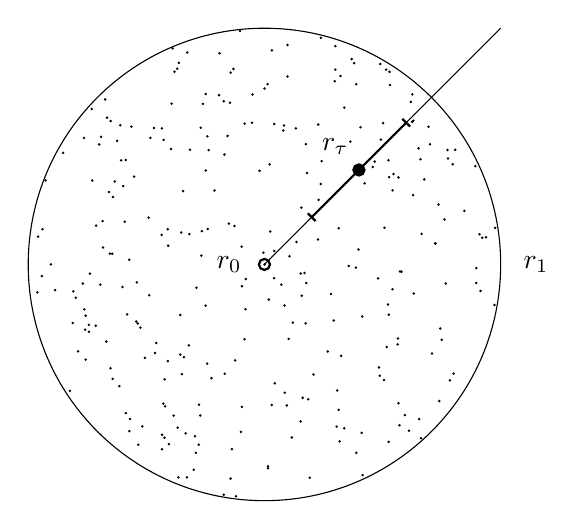
\begin{tikzpicture}[scale=1.5]
			% circles and line
			\draw (0,0) circle (2);
			\draw (0,0) -- (2,2);
			\node[thick] at (0,0) {\pgfuseplotmark{o}};
			%markings fro interval
			\draw[thick] (0.4,0.4) -- (1.2,1.2);
			\node[rotate=45, thick] at (0.4,0.4) {\pgfuseplotmark{|}};
			\node[rotate=45, thick] at (1.2,1.2) {\pgfuseplotmark{|}};
			\node[thick] at (0.8,0.8) {\pgfuseplotmark{*}};
			% labels
			\node at (0.6,1.0) {$r_\tau$};
			\node at (-0.3,0) {$r_0$};
			\node at (2.3,0) {$r_1$};
			% random points
			\foreach \x in {1,...,300}{
				\pgfmathsetmacro{\r}{sqrt(random(0,400)/100)}%
				\pgfmathsetmacro{\a}{random(0,360)}%
				\pgfmathsetmacro{\x}{\r*sin(\a)}
				\pgfmathsetmacro{\y}{\r*cos(\a)}
				\node[fill,circle,inner sep=0pt,minimum size=1pt] at (\x ,\y) {};
			}
		\end{tikzpicture}
	\end{subfigure}
	\begin{subfigure}[t]{0.5\textwidth}
		\centering
		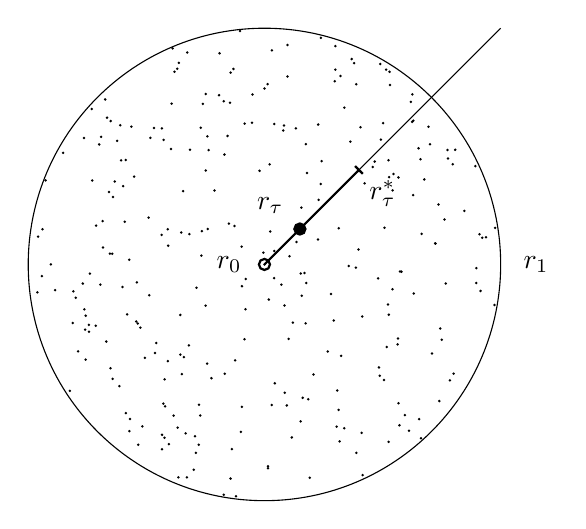
\begin{tikzpicture}[scale=1.5]
			% circles and line
			\draw (0,0) circle (2);
			\draw (0,0) -- (2,2);
			\node[thick] at (0,0) {\pgfuseplotmark{o}};
			%markings fro interval
			\draw[thick] (0.0,0.0) -- (0.8,0.8);
			\node[rotate=45, thick] at (0.8,0.8) {\pgfuseplotmark{|}};
			\node[thick] at (0.3,0.3) {\pgfuseplotmark{*}};
			% labels
			\node at (0.05,0.5) {$r_\tau$};
			\node at (-0.3,0) {$r_0$};
			\node at (2.3,0) {$r_1$};
			\node at (1.0,0.6) {$r_\tau^*$};
			% random points
			\foreach \x in {1,...,300}{
				\pgfmathsetmacro{\r}{sqrt(random(0,400)/100)}%
				\pgfmathsetmacro{\a}{random(0,360)}%
				\pgfmathsetmacro{\x}{\r*sin(\a)}
				\pgfmathsetmacro{\y}{\r*cos(\a)}
				\node[fill,circle,inner sep=0pt,minimum size=1pt] at (\x ,\y) {};
			}
		\end{tikzpicture}
	\end{subfigure}
	\caption{The figure depicts an disk referring to the equilibrium measure when $r_0 = 0$. As the complex plane integral is reduced to a line integral, we draw the domain change and the point of interest $r_\tau$ where $V$ has a critical point. Around this point we depict the region around the minima, which in the method that should account for the main order of the integral we solve for. The left image corresponds to the case when $r_{j/N} >> N^{-\epsilon}$ and the right image corresponds to $r_{j/N} << N^{-\epsilon}$. In this case $r*_{\tau}$ will define the contributing region to the integral.}
\end{figure}

\begin{teorema} 	\label{Theorem: Disk Free Energy}
	For the annulus case, where $r_0 = 0$, we have the following, asymptotically on $N$, for the free energy
	\begin{multline}
		\ln{\pZ{N}{}} = - N^2 I_Q[\mu_Q]  + \frac{1}{2} N \ln N + \frac{N}{2} \left(\ln(2\pi) - 2 - E_Q[\mu_Q]\right) - \frac{5}{12} \ln N \frac{\ln(2\pi)}{2} \\ + \zeta'(-1) + F_V[D_{r_1}] + \Boh(N^{-1/12}(\ln N)^3).
	\end{multline}
	where we have set
	\begin{equation}
		I_Q[\mu_Q] \deff \left[\frac{1}{4} \int_{r_0}^{r_1} q(s) s V^{(2)}(s) \dd s- \ln(r_1) + \frac{1}{2} q(r_1) \right],
	\end{equation}
	\begin{equation}
		E_Q[\mu_Q] \deff \frac{1}{2} \int_{r_0}^{r_1} \ln\left(\frac{V^{(2)}(s)}{4}\right) (sq'(s))' \dd s
	\end{equation}
	and
	\begin{equation}
		F_V[D_{r_1}] \deff \frac{1}{6} \ln{\left(\frac{4}{V^{(2)}_0(0)}\right)} - \frac{1}{3} \ln(r_1) + \frac{5}{32} \ln\left( \frac{V^{(2)}_1(r_1)}{V^{(2)}_{0}(0)} \right) - \frac{1}{32} \frac{r_1  V^{(3)}_1(r_1)}{V^{(2)}_1(r_1)} - \frac{1}{12} \int_{0}^{r_1} \frac{V^{(3)}(r)^2}{V^{(2)}(r)^{2}} r \dd r.
	\end{equation}
\end{teorema}

Again, we start by studying the asymptotic for $h_j$ and then for the summation $\sum \ln(h_j)$. This theorem then should follow from the lemmas concerning this two asymptotics.

\subsection{Asymptotic for the norming constant}

For this subsection, we will focus on getting the asymptotic for the integral
\begin{equation}
	h_j = \int_{\R_+} 2r \ee^{-N V_{\tau(j)}(r)} \dd r
\end{equation}
for each of the degrees $j$. With this, we can proceed to examine the summation over $h_j$ needed top evaluate the free energy as it was shown in \autoref{proposicaoosition: Partition function}. FOr this case however there is one complication. One should distinguish the following two cases depending on a small constant $1/5 > \epsilon > 0$. 

\begin{itemize}
	\item Case 1: $r_{j/N} >> N^{-\epsilon}$. For the annular droplet case where $r_0 > 0$, this case covers all $j = 0, 1, \cdots , N-1$. On the other hand, for the disk droplet case where $r_0 = 0$, this case covers only $j = m_N, m_N + 1, \cdots , N-1$ for $m_N = N^\epsilon$ with some $\epsilon > 0$;
	\item Case 2: $r_{j/N} << N^{-\epsilon}$. This covers the remaining disk droplet case with $j = 0, 1, \cdots, m_N-1$. Notably, the asymptotic expansion involves gamma functions in this case. 
\end{itemize}

We separate this in two proofs, the first one will be regarding $j = m_N, m_N + 1, \cdots, N-1$. One might assume, and would be mainly correct, that nothing is that different in the disk and annulus regimes if the points are distant from $r_0$. The following results are direct adaptations of the previous arguments. 

\begin{teorema}	\label{Theorem: hj disk j>mn}
	For $N-1 \geq j \geq m_N$, asymptotically on $N$,
	\begin{equation}
		h_j =  \frac{\ee^{-N V_{\tau(j)}(r_{\tau(j)})}}{\sqrt{N}} \left( \frac{8\pi r^2_{\tau(j)}}{V^{(2)}_{\tau(j)}(r_{\tau(j)})} \right)^{\frac{1}{2}} \left( 1 + \frac{1}{N} \mathfrak{B}(r_{\tau(j)}) + \epsilon_{N, 1} \right) 
	\end{equation}
	where 
	\begin{equation}
		\mathfrak{B}(r_{\tau(j)}) \deff -\frac{V^{(4)}_{\tau(j)}(r_{\tau(j)})}{V^{(2)}_{\tau(j)}(r_{\tau(j)})^2} \frac{1}{8} - \frac{V^{(3)}_{\tau(j)}(r_{\tau(j)})}{V^{(2)}_{\tau(j)}(r_{\tau(j)})^{2}} \frac{1}{2 r_{\tau(j)}} - \frac{V^{(3)}_{\tau(j)}(r_{\tau(j)})^2}{V^{(2)}_{\tau(j)}(r_{\tau(j)})^{3}} \frac{5}{24},
	\end{equation}
	and
	\begin{equation}
		\epsilon_{N, 1} \deff  \Boh(j^{-\frac{3}{2}} (\ln N)^\alpha)
	\end{equation}
	for some $\alpha > 0$.
\end{teorema}

To actually expand on the details, we need some useful facts. We will make a lot of use of the behavior for $r_\tau$, expressed in \autoref{Proposition: Behavior rt}.

\begin{proposicao} 	\label{Proposition: Behavior rt}
	Due to strict sub-harmonicity of Q in a neighborhood of the droplet, $r_\tau$, defined as before, satisfies 
	\begin{equation}
		r_\tau = \left( \frac{2\tau}{q''(0)} \right)^{\frac{1}{2}} + \Boh(\tau) = \left( \frac{4\tau}{V^{(2)}_0(0)} \right)^{\frac{1}{2}} + \Boh(\tau) 
	\end{equation}
	or more simply
	\begin{equation}
		r_\tau = \Boh \left(\tau^{\frac{1}{2}}\right)
	\end{equation}
	as $\tau \rightarrow 0$.
\end{proposicao}

\begin{proof}
	Begin defining a multivariate function 
	\begin{equation}
		F(\tau, r) = r q'(r) - 2 \tau
	\end{equation}
	such that 
	\begin{equation}
		\begin{cases}
			&F(0, 0) = r q'(r) - 2 \tau =  0, \\
			&\partial_r F(\tau, r) \big|_{(0, 0)} = q'(r) + q''(r) \cdot r \big|_{(0, 0)} = 0
		\end{cases}
	\end{equation}
	since $q$ has critical point at $r_\tau = 0$. This means that the assumptions in the Implicit Function \autoref{Theorem: Implicit Function} do not hold. We must use the \textit{blow-up} technique. Consider a auxiliary variable $v \deff v(r)$ such that $v(r) \tau = r^2 $ and look for solutions of the redefined
	\begin{equation}
		F(\sqrt{v(r) \tau}, \tau) \deff F'(v, \tau) = \frac{\sqrt{v \tau} \cdot q'(\sqrt{v \tau})}{2 \tau} - 1
	\end{equation}
	around $(v_0, 0)$, where $v_0$ is such that $F'(v_0, 0) = 0$. Note that, expanding $q'(r)$ in Taylor around $r=0$ give us
	\begin{equation}
		q'(\sqrt{v \tau}) = q''(0) \cdot \sqrt{v \tau} + \Boh(v \tau),
	\end{equation}
	which, applied in the previous function, 
	\begin{equation}
		F'(v, \tau) = \frac{q''(0)}{2} v - 1 + \Boh(v^{3/2} \tau).
	\end{equation}
	
	Now, we apply the  Implicit Function Theorem on $F'$ noting that the point $v_0$ must satisfy
	\begin{equation}
		v_0 = \frac{2}{q''(0)}
	\end{equation} 
	and that $q''(0) > 0$ by assumption of the global minimum. Then 
	\begin{equation}
		\partial_v F'(v, \tau) \big|_{(v_0, 0)} = \frac{q''(0)}{2} > 0.
	\end{equation}
	 Then, the theorem states that there is a bijective function $v(r\tau) \in C^2$ defined in a neighborhood to $\tau = 0$, for which
	 \begin{equation}
	 	F'(v, \tau) = 0 \quad \text{and} \quad v(0) = v_0.
	 \end{equation}
	 However, $F'(v, \tau) = 0$ means precisely that
	 \begin{equation}
	 	\sqrt{v \tau} \cdot q'(\sqrt{v \tau}) = 2\tau \quad \text{with} \quad r = r(\tau) = \sqrt{v(\tau) \tau}.
	 \end{equation}
	Leading us to believe that locally at $v_0$
	\begin{equation}
		r(\tau) = \left( \frac{2\tau}{q''(0)} \right)^{\frac{1}{2}} + \Boh(\tau)
	\end{equation}
	for some $\tau \rightarrow 0$. Next to zero, all higher powers in the expansion are just order $\tau$.
\end{proof}

To actually go on and prove the stated theorem we start as usual dividing the integral into two sections
\begin{align}
	h_j & = \int_{0}^{\infty} 2 r^{2j + 1} \ee^{-N q(r)} \dd r = \int_{0}^{\infty} 2 r \ee^{-N V_{\tau(j)} (r)} \dd r, \\
	&=\int_{|r - r_{\tau(j)}| < \delta_N} 2 r \ee^{-N V_{\tau(j)}(r)} \dd r+ \int_{|r - r_{\tau(j)}| > \delta_N} 2 r \ee^{-NV_{\tau(j)}(r)} \dd r
	\label{Equation: Separation disk}
\end{align}
 Let's start with a result on the outer integral, which we should be able to control the growth of. 

\begin{lema}  \label{Lemma: mn - N error contributing}
	Consider the case $m_N \leq j \leq N-1$.  If we choose $M$ to be such that
	\begin{equation}
		\int_{|r - r_j| > \delta_N} \left( \ee^{-q(r)} r^{2} \right)^M r \dd r < \infty,
	\end{equation}
	then, for the error-bound integral in which $|r - r_{\tau(j)}| > \delta_N$ we have the asymptotic for $N$ given by
	\begin{equation}
	\int_{|r - r_{\tau(j)}| > \delta_N} 2 r \ee^{-NV_{\tau(j)}(r)} \dd r = \ee^{-N V_{\tau(j)}(r_{\tau(j)})} \Boh\left(\ee^{-c_2 (\ln(N))^2}\right).
	\end{equation}
	for some positive constant $c_2$.
\end{lema}
\begin{proof}
Note that for $d \geq 1$, we choose $C_1$ a constant uniformly for all $\tau$ and write
\begin{equation}
	|V^{(d)}_\tau(r_\tau)| = |q^{(d)}(r_\tau) + (-1)^{d} 2 \tau (d-1)! \ r_\tau^{-d} | \leq C_1 (1 + \tau^{-\frac{d}{2} + 1}).
\end{equation}
Firstly, for $m_N \leq j < N$, we have
\begin{equation}
	r_{\tau(j + 1/2)} - r_{\tau(j)} = \Boh((jN)^{-\frac{1}{2}}).
\end{equation}
Since the potential is increasing in $(r_\tau, \infty)$, the Taylor series expansion for $V_\tau$ is for all $r > r_{\tau(j)} + \delta_N$
\begin{align}	\label{Equation: expansion Vt1/2>}	
	V_{\tau(j +1/2)}(r) & \geq V_{\tau(j +1/2)}(r_{\tau(j)} + \delta_N), \\
	& = V_{\tau(j + 1/2)}(r_{\tau(j +1/2)}) + \frac{1}{2} V^{(2)}_{\tau(j + 1/2)}(r_{\tau(j + 1/2)}) (r_{\tau(j)} + \delta_N - r_{\tau(j + 1/2)})^2 + \Boh(\tau(j)^{-1/2} \delta^3_N).
\end{align}
where $\Boh(\tau(j)^{-1/2} \delta^3_N) = \Boh(N^{-1} j^{-1/2}(\ln(N))^3)$. Similarly, since $V_{\tau}$ is decreasing in $(0, r_\tau)$, we have for all $r < r_{\tau(j)} - \delta_N$
\begin{align}
	V_{\tau(j + 1/2)}(r) & \geq V_{\tau(j +1/2)}(r_{\tau(j)} - \delta_N), \\
	& = V_{\tau(j + 1/2)}(r_{\tau(j + 1/2)}) + \frac{1}{2} V^{(2)}_{\tau(j + 1/2)}(r_{\tau(j + 1/2)}) (r_{\tau(j)} - \delta_N - r_{\tau(j + 1/2)})^2 + \Boh(\tau(j)^{-1/2} \delta^3_N).
	\label{Equation: expansion Vt1/2<}
\end{align}
Using the Taylor series for $V_\tau$ again, we have
\begin{align}
	V_{\tau(j+1/2)}(r_{\tau(j+1/2)}) - V_{\tau(j)}(r_{\tau(j)}) & = V_{\tau(j)}(r_{\tau(j+1/2)}) - V_{\tau(j)}(r_{\tau(j)}) - \frac{1}{N} \ln r_{\tau(j+1/2)}, \\
	& = \Boh((jN)^{-1})  - \frac{1}{N} \ln r_{\tau(j+1/2)}.
\end{align}
Noting that
\begin{equation}
	V_{\tau(j+1/2)}(r_{\tau(j+1/2)}) - V_{\tau(j)}(r_{\tau(j)})
	= [V_{\tau(j+1/2)}(r_{\tau(j+1/2)}) - V_{\tau(j+1/2)}(r)] + [V_{\tau(j+1/2)}(r) - V_{\tau(j)}(r_{\tau(j)})]
\end{equation}
one rewrite using \eqref{Equation: expansion Vt1/2<} and \eqref{Equation: expansion Vt1/2>},
\begin{equation}
	V_{\tau(j+1/2)}(r) - V_{\tau(j)}(r_{\tau(j)}) = - \frac{1}{N} \ln r_{\tau(j+1/2)} + \Boh\left(\frac{\log(N)^2}{N}\right).
\end{equation}

Thus, it follows from the last observations that
\begin{align}
	\ee^{N V_{\tau(j)}(r_{\tau(j)})} & \int_{|r - r_{\tau(j)}| > \delta_N} 2 r^{2j + 1} \ee^{-N q(r)}  \dd r = \int_{|r - r_{\tau(j)}| > \delta_N} 2 \ee^{-N \left( V_{\tau(j + 1/2)}(r) - V_{\tau(j)}(r_{\tau(j)}) \right)} \dd r, \\	
	& = \int_{|r - r_{\tau(j)}| > \delta_N} 2 \ee^{-(N-M) \left( V_{\tau(j + 1/2)}(r) - V_{\tau(j)}(r_{\tau(j)}) \right)} \ee^{-M \left( V_{\tau(j + 1/2)}(r) - V_{\tau(j)}(r_{\tau(j)}) \right)} \dd r, \\	
	& \leq \ee^{-c_1 (\ln(N))^2} \ee^{\frac{N - M}{N} \ln(r_{\tau(j+1/2)})}  \int_{|r - r_{\tau(j)}| > \delta_N} 2 \ee^{-M \left( V_{\tau(j + 1/2)}(r) - V_{\tau(j)}(r_{\tau(j)}) \right)} \dd r, \\
	& = \Boh(\ee^{-c_2 (\ln(N))^2}).
\end{align}
for some constants $c_1, c_2 > 0$ and $M$ such that the integral above converges. The details taken here are very similar to the ones in the annulus case.
\end{proof}


\begin{lema} \label{Lemma: mn - N value contributing}
	Consider the case $m_N \leq j \leq N-1$. For the value-contributing integral we have the asymptotic on $N$ given by
	\begin{equation}
		\int_{|r - r_{\tau(j)}| < \delta_N} 2 r \ee^{-N V_{\tau(j)}(r)} \dd r= \frac{\ee^{-N V_{\tau(j)}}(r_{\tau(j)})}{\sqrt{N}} \left( \frac{8\pi r^2_{\tau(j)}}{V^{(2)}_{\tau(j)}(r_{\tau(j)})} \right)^{\frac{1}{2}} \left( 1 + \frac{1}{N} \mathfrak{B}(r_{\tau(j)}) + \epsilon_{N, 1} \right)
	\end{equation}
	where $\mathfrak{B}(r_{\tau(j)})$ is as in \autoref{Theorem: Disk Free Energy}	and
	\begin{equation}
		\epsilon_{N,1} \deff \Boh(j^{-\frac{3}{2}} (\ln N)^\alpha)
	\end{equation}
	for some $\alpha > 0$.
\end{lema}

\begin{proof}
We now need to examine the integral near the critical point. That is, 
\begin{align}
	& \int_{|r - r_{\tau(j)}| < \delta_N} 2 r \ee^{-N V_{\tau(j)}(r)} \dd r \\
	& =  \ee^{-N V_{\tau(j)}(r_{\tau(j)})} \int_{-\delta_N}^{\delta_N} 2(r_{\tau(j)} + t) \ee^{-N \left( \frac{1}{2} V^{(2)}_{\tau(j)}(r_{\tau(j)}) (t)^2 + \frac{1}{3!} V^{(3)}_{\tau(j)}(r_{\tau(j)}) (t)^3 + \frac{1}{4!} V^{(4)}_{\tau(j)}(r_{\tau(j)}) (t)^4 + \Boh(\tau(j)^{-\frac{3}{2}}  t^5) \right)} \dd t, \\
	&  
	\begin{multlined}
	=  \ee^{-N V_{\tau(j)}(r_{\tau(j)})}  \int_{-\sqrt{N} \delta_N}^{\sqrt{N} \delta_N} 2 \ee^{-\frac{1}{2} V^{(2)}_{\tau(j)}(r_{\tau(j)}) t^2} \left(r_{\tau(j)} + \frac{t}{\sqrt{N}}\right)  \left(  1 - \frac{V^{(3)}_{\tau(j)}(r_{\tau(j)}) t^3 }{6 \sqrt{N}} \right. \\ \left. - \frac{V^{(4)}_{\tau(j)}(r_{\tau(j)}) t^4}{24 N}  + \frac{V^{(3)}_{\tau(j)}(r_{\tau(j)})^2 t^6}{72 N} + \epsilon_{N,1} \right) \dd t,
	\end{multlined}
\end{align}
where  $\epsilon_{N,1} = \Boh(j^{-\frac{3}{2}} (\ln N)^\alpha)$ for some $\alpha > 0$. From here, the expression is directly identified with \eqref{Equation: value-contributing integral} and the techniques for getting the result are one-to-one with the ones already done in that case.
then, distributing the integral,
\begin{multline}
	\int_{|r - r_{\tau(j)}| < \delta_N} 2 r \ee^{-N V_{\tau(j)}(r)} \dd r  \\ = 2 r_{\tau(j)} \frac{\ee^{-N V_{\tau(j)}(r_{\tau(j)})}}{\sqrt{N}}
\left[
\left(- \frac{V^{(4)}_{\tau(j)}(r_{\tau(j)})}{24 N} - \frac{V^{(3)}_{\tau(j)}(r_{\tau(j)})}{6 r_{\tau(j)} N} \right)
\int_{-\ln(N)}^{\ln(N)} \ee^{-\frac{y^2}{2} V^{(2)}_{\tau(j)}(r_{\tau(j)})} y^4 \dd y \right. \\
\left. - \frac{V^{(3)}_{\tau(j)}(r_{\tau(j)})^2}{72 N}
\int_{-\ln(N)}^{\ln(N)} \ee^{-\frac{y^2}{2} V^{(2)}_{\tau(j)}(r_{\tau(j)})} y^6 \dd y +
\int_{-\ln(N)}^{\ln(N)} \ee^{-\frac{y^2}{2} V^{(2)}_{\tau(j)}(r_{\tau(j)})} \dd y + \epsilon_{N,1} \right].
\end{multline}
At this point, the result is directly evaluated using the Gaussian integrals in \autoref{Prop: Gaussian integrals}.	So that we finally substitute the values to get
\begin{multline}
		\int_{|r - r_{\tau(j)}| < \delta_N} 2 r \ee^{-N V_{\tau(j)}(r)} \dd r  \\ = \sqrt{2\pi} r_{\tau(j)} \frac{\ee^{-N V_{\tau(j)}(r_{\tau(j)})}}{\sqrt{N}} \left[
	\left(- \frac{V^{(4)}_{\tau(j)}(r_{\tau(j)})}{24 N} - \frac{V^{(3)}_{\tau(j)}(r_{\tau(j)})}{6 r_{\tau(j)} N} \right) \frac{3}{16} \left( \frac{4}{V^{(2)}_{\tau(j)}(r_{\tau(j)})} \right)^{\frac{5}{2}} \right. \\
	\left. - \frac{V^{(3)}_{\tau(j)}(r_{\tau(j)})^2}{72 N} \frac{15}{64} \left(\frac{4}{V^{(2)}_{\tau(j)}(r_{\tau(j)})} \right)^{\frac{7}{2}} +
	\left( \frac{4}{V^{(2)}_{\tau(j)}(r_{\tau(j)})} \right)^{\frac{1}{2}} + \epsilon_{N,1} \right],
\end{multline}
and, rearranging the terms we should get our result.
\end{proof}

\begin{proof} (\autoref{Theorem: hj disk j>mn})
	This is now only a matter to notice that the expression derived in \autoref{Lemma: mn - N error contributing} is absolved in to the error term of the expression in \autoref{Lemma: mn - N value contributing} and the result follows.
\end{proof}

So far, nothing is considerably different from both cases as we are dealing with point distant from the origin. We must now deal with the more delicate case, for $j \leq m_N$. The behavior for $h_j$, in this regimen, is expressed by the following theorem.

\begin{teorema}	\label{Theorem: hj disk j<mn}
	For $0 \leq j < m_N$, we will have the following asymptotic for the norming constant
	\begin{equation}
	 h_j =  \ee^{-N q(0)} \left[ N^{-(j+1)} \Gamma(j+1)\left(\frac{1}{2} q''(0)\right)^{-(j+1)} \left( 1 + \Boh(N^{-\frac{1}{2}} (j+1/2)^{\frac{3}{2}} (\ln N)^3) \right)+ \epsilon_N(j) \right]
	\end{equation}
	where $\Gamma$ is the usual Gamma function and 
	\begin{equation}
		\epsilon_N(j) \deff \Boh\left(\ee^{-c_2 (j + 1) (\ln N)^2}  \left(\frac{j+1}{N} (\ln(N))^2 \right)^{(j+1) \frac{N-M}{N}} \right)
	\end{equation}
	with $c_2 > 0$ a constant.
\end{teorema}

\begin{proof}
For $j < m_N$, we need to define some $r^*_\tau \deff r_\tau \ln(N)$ from which we separate the integral in a important part close to the origin and another part which has a lesser order. Consider then the decomposition
\begin{equation}
	h_j = \int_{0}^{\infty} 2r^{2j+1} \ee^{-N q(r)} \dd r =\int_{0}^{r^*_{\tau(j+1)}} 2r^{2j+1} \ee^{-N q(r)} \dd r + \int_{r^*_{\tau(j+1)}}^{\infty} 2r^{2j+1} \ee^{-N q(r)} \dd r.
\end{equation}
Due to strict sub-harmonicity of Q in a neighborhood of the droplet, $r_\tau$ satisfies $r_\tau = \Boh (\tau^{\frac{1}{2}})$ as $\tau \rightarrow 0$, this is given by \autoref{Proposition: Behavior rt}. Since $V_\tau$ has a global minimum at $r = r_\tau$ and increases for larger values, for all $r > r^*_{\tau(j + 1)}$ we have
\begin{align}
	V_{\tau(j+1/2)}(r) & \geq V_{\tau(j+1)}(r)(r^*_{\tau(j+1)}) = q(r^*_{\tau(j+1)}) - \frac{2j + 1}{N} \ln(r^*_{\tau(j+1)}), \\
	& = q(0) + \frac{1}{2} q''(0)(r^*_{\tau(j+1)})^2 - \frac{2j + 1}{N} \ln(r^*_{\tau(j+1)}) + \Boh(r^*_{\tau(j+1)})^3.
\end{align}
Note that $q'(0) = 0$ since $\Delta Q(z) \in (0, \infty)$ near the origin and $\Delta Q(z) \propto q'(0)/r + q''(0)$. Take
\begin{align}
	\ee^{-N q(0)} \int_{r^*_{\tau(j+1)}}^{\infty} 2r^{2j+1} \ee^{-N q(r) + N q(0)} \dd r & =  \ee^{-N q(0)} \int_{r^*_{\tau(j+1)}}^{\infty} 2 \ee^{(2j+1) \ln(r) -N q(r) + N q(0)} \dd r, \\
	& = \ee^{-N q(0)} \int_{r^*_{\tau(j+1)}}^{\infty} 2 \ee^{- N \left(-\frac{2}{N}\left( j + \frac{1}{2} \right) \ln(r) - q(r) + q(0)\right)} \dd r, \\
	& = \int_{r^*_{\tau(j+1)}}^{\infty} 2 \ee^{-N (V_{\tau(j+1/2)}(r) - q(0))} \dd r
\end{align}
and, using the inequality explicited above
\begin{align}
	\ee^{- N V_{\tau(j+1)}(r) + N q(0)} & = \ee^{- N V_{\tau(j+1)}(r) + N q(0) + M V_{\tau(j+1)}(r) - M V_{\tau(j+1)}(r)}, \\
	& = \ee^{- (N - M) V_{\tau(j+1)}(r) + N q(0) - M V_{\tau(j+1)}(r)}, \\
	& \leq \ee^{- (N - M) V_{\tau(j+1)}(r^*) + N q(0) - M V_{\tau(j+1)}(r)}, \\
	& = \ee^{- (N - M) \left(V_{\tau(j+1)}(r^*) - q(0) \right)} \ee^{- M \left(V_{\tau(j+1)}(r) - q(0) \right)}.
\end{align}
Then
\begin{align}
	&  \int_{r^*_{\tau(j+1)}}^{\infty} 2 \ee^{-N (V_{\tau(j+1)}(r) - q(0))} \dd r \\
	& \leq  \ee^{ - (N - M) V_{\tau(j+1)}(r^*)} \ee^{(N-M) q(0)}\int_{r^*_{\tau(j+1)}}^{\infty} 2 \ee^{-M V_{\tau(j+1)}(r) } \dd r, \\
	& =  \ee^{ - (N - M) \left[ q(r^*_{\tau(j+1)}) - \frac{2j+2}{N} \ln(r^*_{\tau(j+1)}) \right]} \ee^{(N-M) q(0)} \int_{r^*_{\tau(j+1)}}^{\infty} 2 \ee^{-M V_{\tau(j+1)}(r) } \dd r, \\
	& = \ee^{- (N-M) q(r^*_{\tau(j+1)})} {r^*_{\tau(j+1)}}^{(2j+2) \frac{N-M}{N}} \ee^{(N-M) q(0)} \int_{r^*_{\tau(j+1)}}^{\infty} 2 \ee^{-M V_{\tau(j+1)}(r) } \dd r, \\
	& = \ee^{- (N-M) \left[\frac{q''(0)}{2}  (r^*_{\tau(j+1)})^2 + \Boh(r^*_{\tau(j+1)})^3\right] } {r^*_{\tau(j+1)}}^{(2j+2) \frac{N-M}{N}} \int_{r^*_{\tau(j+1)}}^{\infty} 2 \ee^{-M V_{\tau(j+1)}(r)} \dd r, \\
	& \leq \ee^{- \frac{(N-M)}{2} q''(0) (r^*_{\tau(j+1)})^2)} {r^*_{\tau(j+1)}}^{(2j+2)\frac{N-M}{N}} \int_{r^*_{\tau(j+1)}}^{\infty} 2 \ee^{-M V_{\tau(j+1)}(r)} \dd r, \\
	& = \ee^{- c_1 \frac{(N-M)}{2}r_{\tau(j+1)}^2 \ln(N)^2} {r^*_{\tau(j+1)}}^{(2j+2)\frac{N-M}{N}} \int_{r^*_{\tau(j+1)}}^{\infty} 2 \ee^{-M V_{\tau(j+1)}(r)} \dd r \deff \epsilon_N(j) \\
\end{align}
for some $c_1 > 0$ and $M$ as given in the other proof such that the integral converges.  Since $r_\tau = \Boh(\tau^{\frac{1}{2}})$, there is a constant $c_2 > 0$ such that as $N$ goes to infinity
\begin{align}
	\epsilon_N(j)  & = \Boh \left(\ee^{- c_1 \frac{(N-M)}{2} \tau(j+1) \ln(N)^2} {r^*_{\tau(j+1)}}^{(2j+2)\frac{N-M}{N}}\right), \\
	&= \Boh \left(\ee^{- c_2 (j+1) \ln(N)^2} {r^*_{\tau(j+1)}}^{(2j+2)\frac{N-M}{N}}\right), \\
	& = \Boh\left(\ee^{-c_2 (j + 1) (\ln N)^2}  \left(\frac{j+1}{N} (\ln(N))^2 \right)^{(j+1) \frac{N-M}{N}} \right).
\end{align}

Therefore we obtain
\begin{align}
	h_j & = \int_{0}^{\infty} 2r^{2j+1} \ee^{-N q(r)} \dd r = \int_{0}^{r^*_{\tau(j+1)}} 2r^{2j+1} \ee^{-N q(r)} \dd + \ee^{-N q(0)} \epsilon_N(j), \\
	& = \int_{0}^{r^*_{\tau(j+1)}} 2r^{2j+1} \ee^{-N \left( q(0) + \frac{1}{2} q''(0) r^2 \right) + \Boh(N(r^*_{\tau(j+1)})^3)} \dd  r + \ee^{-N q(0)} \epsilon_N(j), \\
	& =  \ee^{-N q(0)} \left[ \int_{0}^{r^*_{\tau(j+1)}} 2r^{2j+1} \ee^{-\frac{1}{2} q''(0) r^2 N} \dd r \left( 1 + \Boh(N(r^*_{\tau(j+1)})^3) \right)+ \epsilon_N(j) \right], \\
	&=  \ee^{-N q(0)} \left[ N^{-(j+1)} \Gamma(j+1)\left(\frac{1}{2} q''(0)\right)^{-(j+1)} \left( 1 + \Boh(N^{-\frac{1}{2}} (j+1/2)^{\frac{3}{2}} (\ln N)^3) \right)+ \epsilon_N(j) \right]
\end{align}
where $\Gamma$ is the usual gamma function with integral representation
\begin{equation}
	\Gamma(j+1) = \int_{0}^{\infty} t^j \ee^{-t} \dd t
\end{equation}
and we used $t = 1/2 q''(0) r^2 N$.
  
\end{proof}

\subsection{Asymptotics on the Summation}

So now we need to return to  \eqref{Equation: Partition Function} and calculate each term for $	\sum_{j=0}^{N-1} \ln{h_j}$ using the expansion in terms of \autoref{Theorem: hj disk j>mn} and \autoref{Theorem: hj disk j<mn} for the expression

\begin{equation}
	\sum_{j=0}^{N} \ln(h_j) = \sum_{j=0}^{m_N - 1} \ln(h_j)  + \sum_{j=m_N}^{N - 1} \ln(h_j).
\end{equation}

\begin{teorema}	\label{Theorem: Disk sum}
	We have the following asymptotics on $N$ for the summation of $\ln(h_j)$ from $0$ to $N - 1$,
	\begin{multline}
		\sum_{j=0}^{N-1} \ln (h_j) = -N^2 I[\mu_Q] - \frac{1}{2} N \ln(N)  -\frac{N}{2} \left( E_Q[\mu_Q] - \ln(2\pi) \right) - \frac{\ln(N)}{12} \\ + \zeta'(-1) + F_V[D_{r_1}] + \Boh(N^{-12} (\ln N)^3)
		% - N^2 I_Q[\mu_Q]  -\frac{1}{2} N \ln N - \frac{N}{2} \left(E_Q[\mu_Q] - \ln(8\pi) \right) \\ - \frac{\ln N}{12} + \zeta'(-1) + F_Q[D_{r_1}] + \Boh(N^{-1/12}(\ln N)^3)
	\end{multline}
	where $I_Q[\mu_Q] $, $F_V[D_{r_1}]$ and $E_Q[\mu_Q]$ are as in \autoref{Theorem: Disk Free Energy}.
	%and
	%\begin{equation}
	%	F_Q[D_{r_1}] \deff \frac{1}{12} \ln{\frac{1}{r_1^2 V^{(2)}_1(r_1)}} - \frac{1}{16} \left( r_1 \frac{V^{(3)}_1(r_1)}{V^{(r_1)}} \right) + \frac{1}{24} \int_{0}^{r_1} \left( \frac{V^{(3)}(r)}{V^{(2)}(r)}\right)^2 r \dd r.
	%\end{equation}
\end{teorema}

To prove this theorem, we must give the asymptotics for both summations. This means we need both \autoref{Lemma: Summation disk <mn}, referring to the sum from powers $0$ to $m_N-1$, and \autoref{Lemma: Summation disk >mn}, referring to the sum from $m_N$ to $N-1$. We start by the lower power terms.

\begin{lema}	\label{Lemma: Summation disk <mn}
	We have the following asymptotic for the summation of $\ln(h_j)$ from $0$ to $m_N - 1$,
	\begin{multline}
		\sum_{j=0}^{m_N - 1} \ln(h_j)  = -m_N N q(0) - \frac{m_N(m_N + 1)}{2} \left( \ln(N) + \ln\left( \frac{1}{2} q''(0) \right)  \right) +  \frac{m_N^2 \ln(m_N)}{2} - \frac{3}{4} m_N^2 \\ + \frac{\ln(2\pi) m_N}{2} - \frac{\ln(m_N)}{12} + \zeta'(-1)+ \Boh(m_N^{-2}+ N^{-\frac{1}{2}(1-5\epsilon)} (\ln(N))^3).
	\end{multline}
	where $\epsilon$ is as in the definition for $m_N$.
\end{lema}

\begin{proof}

The first term in the right is straightforwardly determined, we need only to write, using \autoref{Theorem: hj disk j<mn},
\begin{align}
	&
	\begin{multlined}
	\sum_{j=0}^{m_N - 1} \ln(h_j) = -m_N N q(0) - \frac{m_N(m_N + 1)}{2} \left( \ln(N) + \ln\left( \frac{1}{2} q^{(2)}(0) \right) \right) \\ + \ln(G(m_N + 1)) + \Boh(N^{-\frac{1}{2}(1-5\epsilon)} (\ln(N))^3),
	\end{multlined} \\
	& 
	\begin{multlined}
		= -m_N N q(0) - \frac{m_N(m_N + 1)}{2} \left( \ln(N) + \ln\left( \frac{1}{2} q^{(2)}(0) \right)  \right) +  \frac{m_N^2 \ln(m_N)}{2} - \frac{3}{4} m_N^2 \\ + \frac{\ln(2\pi) m_N}{2} - \frac{\ln(m_N)}{12} + \zeta'(-1)+ \Boh(m_N^{-2}+ N^{-\frac{1}{2}(1-5\epsilon)} (\ln(N))^3)
	\end{multlined}
\end{align}
where $G$ is the Barnes $G$-function defined recursively as
\begin{equation}
	G(z+1) = \Gamma(z) G(z),
\end{equation}
and we have used the asymptotic for the G-Barnes function
\begin{equation}
	\ln(G(z+1)) = \frac{z^2 \ln(z)}{2} - \frac{3}{4} z^2 + \frac{\ln(2\pi) z}{2} - \frac{\ln(z)}{12} + \zeta'(-1) + \Boh\left(\frac{1}{z^2}\right).
\end{equation}
\end{proof}

\begin{lema}	\label{Lemma: Summation disk >mn}
	We have the following asymptotic for the summation of $\ln(h_j)$ from $m_N$ to $N-1$,
	\begin{multline}
		\sum_{j=m_N}^{N-1} \ln (h_j) = -N^2 I[\mu_Q] + \frac{(N-m_N)}{2} \ln{\frac{2\pi}{N}} +  N m_N q(0) + \frac{3}{4} m_N^2 - \frac{N}{2} E_Q[\mu_Q] \\ - \frac{m_N}{2} \left(m_N + 1\right) \ln{\left(\frac{4}{V^{(2)}_0(0)}\right)} - \frac{1}{2} \left( m_N^2 - \frac{1}{6} \right) \ln{\left(\frac{m_N}{N}\right)} + F_V[D_{r_1}] + \Boh(N^{-12} (\ln N)^3),
	\end{multline}
	where $I_Q[\mu_Q] $,  $F_V[D_{r_1}]$ and $E_Q[\mu_Q]$ are as in \autoref{Theorem: Disk Free Energy}.
\end{lema}

The second summation is a bit more detailed, we use the previously defined asymptotics in \autoref{Theorem: hj disk j>mn},
\begin{equation}
	\ln(h_j) = -N V_{\tau(j)} (r_{\tau(j)}) + \frac{1}{2} \ln{\left( \frac{8\pi r^2_{\tau(j)}}{N V^{(2)}_{\tau(j)}(r_{\tau(j)})}  \right)} + \frac{1}{N} \mathfrak{B}(r_{\tau(j)}) + \Boh(j^{-\frac{3}{2}} (\ln(N))^\alpha)
\end{equation}
and need to determine the asymptotic of three terms in order to get the full summation,
\begin{align}
	& -N\sum_{j=m_N}^{N-1} V_{\tau(j)}(r_{\tau(j)}), \quad \sum_{j=m_N}^{N-1} \ln \left( \frac{V^{(2)}_{\tau(j)}(r_{\tau(j)})}{4}\right)  \quad \text{and} \quad \sum_{j=m_N}^{N-1}  \ln(r_{\tau(j)}).
\end{align}
This is done in \autoref{Proposition: mn-N v disk}, \autoref{Proposition: mn-N lnv disk} and \autoref{Proposition: mn-N lnr disk}.

\begin{proposicao}	\label{Proposition: mn-N v disk}
	The following asymptotic holds under the same context as \autoref{Lemma: Summation disk >mn}.
	\begin{multline}
		-N \sum_{j=m_N}^{N-1} V_{\tau(j)}(r_{\tau(j)}) = -N^2 I_Q[\mu_Q]  + N U_{\mu_Q}(0) + \frac{1}{6} \ln(r_1) + N m_N q(0) + \frac{3}{4} m_N^2 \\ - \frac{1}{2} \left(m_N^2 - m_N + \frac{1}{6} \right) \ln{\left(\frac{4 m_N}{N V^{(2)}_0(0)}\right)} - \frac{m_N}{2} + \Boh{\left(N^{-\frac{1}{2}(3-5\epsilon)}\right)}.
	\end{multline}
	Here, $I_Q[\mu_Q] $ is as in \autoref{Theorem: Disk Free Energy}, $\epsilon$ is as in the definition for $m_N$, and
	\begin{equation}
		 2 U_{\mu_Q}(0) \deff q(r_1) - 2 \ln(r_1) - q(0).
	\end{equation}
\end{proposicao}

\begin{proof}
We proceed as before and use the Euler-Maclaurin formula to write
\begin{multline}
	\sum_{j=m_N}^{N-1} V_{\tau(j)}(r_{\tau(j)}) = \int_{m_N}^N V_{\tau(t)}(r_{\tau(t)})  \dd t - \frac{1}{2} \left( V_{\tau(N)}(r_{\tau(N)})  - V_{\tau(m_N)}(r_{\tau(m_N)}) \right) + \\ \frac{1}{12} \left[ \partial_t V_{\tau(t)}(r_{\tau(t)}) |_{t=N} - \partial_t V_{\tau(t)}(r_{\tau(t)}) |_{t=m_N} \right] + \Boh(N^{-3}).
	\label{Equation: EulerMaclaurin 1 disk}
\end{multline}
Then, we are able to rewrite, setting $s = r_{\tau(j)}$,
\begin{align}
	\int_{m_N}^N V_{\tau(t)}(r_{\tau(t)})  \dd t & = \int_{m_N}^N (q(r_{\tau(t)}) - 2 \tau(t) \ln(r_{\tau(t)})) \dd t, \\
	& = \frac{1}{2} \int_{r_{\tau(m_N)}}^{r_1} (q(s) - s q'(s) \ln(s)) s V^{(2)}(s) N \dd s, \\
	& = N \left[  \frac{1}{2} \int_{r_{\tau(m_N)}}^{r_1} q(s) s V^{(2)}(s) \dd s -  \frac{1}{2} \int_{r_{\tau(m_N)}}^{r_1} s^2 q'(s) \ln(s) V^{(2)}(s) \dd s \right].
\end{align}
Using that $r_1 q'(r_1) = 2$, apply integration by parts on the second term and get
\begin{align}
	& \frac{1}{2} \int_{r_{\tau(m_N)}}^{r_1} s^2 q'(s) \ln(s) V^{(2)}(s) \dd s \\
	& = \frac{1}{2} \int_{r_{\tau(m_N)}}^{r_1} s^2 q'(s) \ln(s) \frac{1}{s} (s q'(s))' \dd s, \\
	& = \frac{1}{4} \int_{r_{\tau(m_N)}}^{r_1} ((sq'(s))^2)' \ln(s) \dd s, \\
	& = \frac{1}{4} (s q'(s))^2 \ln(s) |_{r_{\tau(m_N)}}^{r_1} - \frac{1}{4}  \int_{r_{\tau(m_N)}}^{r_1} (s q'(s))^2 \frac{1}{s} \dd s, \\
	& = \ln(r_1) - \frac{1}{4} \int_{r_{\tau(m_N)}}^{r_1} s q'(s)^2 \dd s - \frac{m_N^2}{N^2} \ln(r_{\tau(m_N)}), \\
	& = \ln(r_1) - \frac{1}{4} (s q'(s) q(s)) |_{r_{\tau(m_N)}}^{r_1} + \frac{1}{4} \int_{r_{\tau(m_N)}}^{r_1} q(s) (s q'(s))' \dd s  - \frac{m_N^2}{N^2} \ln(r_{\tau(m_N)}), \\
	& = \ln(r_1) - \frac{1}{2} q(r_1) + \frac{1}{4} \int_{r_{\tau(m_N)}}^{r_1} q(s) (s q'(s))'\dd s  - \frac{m_N^2}{N^2} \ln(r_{\tau(m_N)}) + \frac{m_N}{2 N} q(r_{\tau(m_N)}).
\end{align}
Leaving us with
\begin{align}
	& \begin{multlined}
		N \left[\frac{1}{4} \int_{r_{\tau(m_N)}}^{r_1} q(s) s V^{(2)}(s) \dd s - \ln(r_1) + \frac{1}{2} q(r_1) - \frac{m_N^2}{N^2} \ln(r_{\tau(m_N)}) + \frac{m_N}{2 N} q(r_{\tau(m_N)})  \right] 
	\end{multlined} \\
	& \deff N I_Q[\mu_Q]  - \frac{1}{4} \int_{r_0}^{r_{\tau(m_N)}} q(s) s  V^{(2)}(s) \dd s  - \frac{m_N^2}{N} \ln(r_{\tau(m_N)}) + \frac{m_N}{2} q(r_{\tau(m_N)}).
	\label{Equation: Equilibrium energy disk}
\end{align}
where we expand some terms using the following results given by \autoref{Proposition: Behavior rt}
\begin{equation}
	\ln(r_{\tau(m_N)}) = \frac{1}{2} \ln{\left(\frac{4 \tau(m_N)}{V^{(2)}_0(0)}\right)} + \Boh(\tau(m_N)^{\frac{1}{2}}) = \frac{1}{2} \ln{\left(\frac{4 \tau(m_N)}{V^{(2)}_0(0)}\right)} + \Boh(N^{-\frac{1}{2}(1-\epsilon)}),
	\label{Equation: behavior ln rt mn}
\end{equation}
\begin{equation}
	q(r_{\tau(m_N)}) = q(0) + \frac{1}{2} q''(0)(r_{\tau(m_N)})^2 + \Boh((\tau(m_N)^{\frac{3}{2}})) = q(0) + \tau(m_N) + \Boh(N^{-\frac{3}{2}(1 - \epsilon)}),
	\label{Equation: behavior q(rt)}
\end{equation}
and, using integration by parts we solve the integral
\begin{align}
	 \frac{1}{4} \int_{r_0}^{r_{\tau(m_N)}} q(s) s  V^{(2)}(s) \dd s  & =
	  \frac{1}{4} \int_{r_0}^{r_{\tau(m_N)}} q(s) (s q'(s))' \dd s, \\
	  & = \frac{1}{2} \tau(m_N) q(r_{\tau(m_N)}) - \frac{1}{4} \int_{0}^{r_{\tau(m_N)}} s (q'(s))^2 \dd s, \\
	  & = \frac{1}{2} \tau(m_N) q(r_{\tau(m_N)})  - \frac{1}{4} (q''(0))^2  \int_{0}^{r_{\tau(m_N)}} s^3 \dd s + \Boh{(r^5_{\tau(m_N)})}, \\
	  & = \frac{1}{2} \tau(m_N) q(r_{\tau(m_N)}) - \frac{1}{4} \tau(m_N)^2 + \Boh(N^{-5/2(1-\epsilon)}).
\end{align}
Therefore, for this first term, gathering the above and expanding using \autoref{Proposition: Behavior rt} and \eqref{Equation: behavior q(rt)},
\begin{align}
	& \begin{multlined}
			\int_{m_N}^N V_{\tau(t)}(r_{\tau(t)})  \dd t  = N I_Q[\mu_Q]  -  \frac{1}{2} \tau(m_N) q(r_{\tau(m_N)}) - \frac{1}{4} \tau(m_N)^2 + \Boh(N^{-5/2(1-\epsilon)}) \\ - \frac{m_N^2}{2N} \ln{\left(\frac{4 \tau(m_N)}{V^{(2)}_0(0)}\right)}  + \Boh(N^{-\frac{3}{2}(1 - \epsilon)}) + \frac{m_N}{2} \left(q(0) + \tau(m_N)  \right) + \Boh(N^{-\frac{1}{2}(1-\epsilon)}),
	\end{multlined} \\
	& = N I_Q[\mu_Q]  - m_N q(0) - \frac{3}{4} \frac{m_N^2}{N} + \frac{m_N^2}{2N} \ln{\left( \frac{4 m_N}{N V^{(2)}_0(0)} \right)} + \Boh{\left(N^{-\frac{1}{2}(3-5\epsilon)}\right)}.
\end{align}

For the other terms in the Euler-Maclaurin formula we have
\begin{align}
	V_{\tau(N)}(r_{\tau(N)})  &- V_{\tau{(m_N)}}(r_{\tau(m_N)}) = q(r_1) - 2 \ln(r_1) - q(r_{\tau(m_N)}) + 2 \tau(m_N) \ln(r_{\tau(m_N)}), \\
	& = q(r_1) - 2 \ln(r_1) - q(0) - \frac{m_N}{N} + \frac{m_N}{N} \ln{\left(\frac{4 m_N}{N V^{(2)}_0(0)}\right)} + \Boh(N^{-3/2(1-\epsilon)}), \\
	& \deff 2 U_{\mu_Q}(0) - \frac{m_N}{N} + \frac{m_N}{N} \ln{\left(\frac{4 m_N}{N V^{(2)}_0(0)}\right)} + \Boh(N^{-3/2(1-\epsilon)}),
\end{align}
and,
\begin{align}
		\partial_t (V_{\tau(t)}(r_{\tau(t)})) |_{t=N} - \partial_t (V_{\tau(t)}(r_{\tau(t)})) |_{t=m_N} & = \frac{2}{N}(\ln(r_{\tau(m_N)}) - \ln(r_1)), \\
		& = \frac{1}{N} \ln{\left(\frac{4 m_N}{N V^{(2)}_0(0)}\right)}  - \frac{2}{N} \ln(r_1) + \Boh(N^{-1/2(3-\epsilon)}).
\end{align}

Finally, gathering terms, we get the lemma.
\end{proof}

\begin{proposicao}	\label{Proposition: mn-N lnv disk}
	We have following asymptotic
	\begin{equation}
		\sum_{j=m_N}^{N-1}\ln \left( \frac{V^{(2)}_{\tau(j)}(r_{\tau(j)})}{4}\right) = N E_Q(\mu_Q)  - \frac{1}{2} \ln \left( \frac{V^{(2)}_{1}(r_1)}{V^{(2)}_{0}(r_{0})} \right)  - m_N \ln\left(  \frac{V^{(2)}_0(0)}{4} \right) + \Boh(N^{-1/2(1-\epsilon)}),
	\end{equation}
	where $E_Q[\mu_Q]$ is as in \autoref{Theorem: Disk Free Energy} and $\epsilon$ is as in the definition for $m_N$.
\end{proposicao}
\begin{proof}
	Again, we start with the Euler-Maclaurin formula
		\begin{multline}
		\sum_{j=m_N}^{N-1} \ln \left( \frac{V^{(2)}_{\tau(j)}(r_{\tau(j)})}{4}\right) = \int_{m_N}^{N} \ln \left( \frac{V^{(2)}_{\tau(t)}(r_{\tau(t)})}{4}\right)  \dd t - \frac{1}{2} \ln \left( \frac{V^{(2)}_{1}(r_1)}{V^{(2)}_{\tau(m_N)}(r_{\tau(m_N)})} \right) + \\ \frac{1}{12} \left[ \partial_t \ln \frac{1}{4} V^{(2)}_{\tau(t)}(r_{\tau(t)}) |_{t=N} - \partial_t \ln \frac{1}{4} V^{(2)}_{\tau(t)}(r_{\tau(t)}) |_{t=m_N}\right]  + \Boh(N^{-3}).
	\end{multline}
	We first tackle the integral on the right hand side. Changing variables $s = r_{\tau(t)}$ we have
	\begin{align}
		\int_{m_N}^{N} \ln \left( \frac{V^{(2)}_{\tau(t)}(r_{\tau(t)})}{4}\right)  \dd t & = \frac{N}{2} \int_{r_{\tau(m_N)}}^{r_1} \ln\left(\frac{V^{(2)}(s)}{4}\right) (sq'(s))' \dd s, \\
		& =  \frac{N}{2} \int_{r_{\tau(m_N)}}^{r_1} \ln\left(\frac{V^{(2)}(s)}{4}\right)  s V^{(2)}(s) \dd s, \\
		& = \frac{N}{2} \left[ \int_{r_0}^{r_1}\ln\left(\frac{V^{(2)}(s)}{4}\right) s V^{(2)}(s) \dd s -  \int_{r_0}^{r_{\tau(m_N)}} \ln\left(\frac{V^{(2)}(s)}{4}\right) s V^{(2)}(s) \dd s  \right], \\
		& = \frac{N}{2} \left[ 2 E_Q[\mu_Q] -  \int_{r_0}^{r_{\tau(m_N)}} \ln\left(\frac{V^{(2)}(s)}{4}\right) s V^{(2)}(s) \dd s  \right], 
	\end{align}
	where one also compute
	\begin{align}
		\int_{r_0}^{r_{\tau(m_N)}} & \ln\left(\frac{V^{(2)}(s)}{4}\right) s V^{(2)}(s) \dd s \\ 
		& = \int_{r_0}^{r_{\tau(m_N)}} \ln\left(\frac{V^{(2)}_0(0)}{4} + \frac{V^{(2)}_0(0)}{4} s + \Boh(s^2) \right) s \left( V^{(2)}_0(0) + V^{(2)}_0(0) s + \Boh(s^2) \right) \dd s, \\
		& = \int_{r_0}^{r_{\tau(m_N)}} \ln\left( \frac{V^{(2)}_0(0)}{4} \right) s V^{(2)}_0(0)  \dd s + \Boh(r_{\tau(m_N)}^3), \\
		& =  \ln\left( \frac{V^{(2)}_0(0)}{4} \right) r_{\tau(m_N)}^2 V^{(2)}_0(0) + \Boh(r_{\tau(m_N)}^3), \\
		& = \frac{2m_N}{N}\ln\left( \frac{V^{(2)}_0(0)}{4} \right)  + \Boh(N^{-3(1-\epsilon)}) 
	\end{align}
	noting the definition for $V$ and \autoref{Proposition: Behavior rt}. Furthermore, we know 
	\begin{align}
		\partial_t \ln \frac{1}{4}V^{(2)}_{\tau(t)}(r_{\tau(t)}) & = \partial_V \left( \ln \frac{1}{4} V^{(2)}_{\tau(t)}(r_{\tau(t)}) \right)  \frac{1}{4}  \partial_r \left( V^{(2)}_{\tau(t)}(r_{\tau(t)}) \right) \partial_\tau \left( r_{\tau(t)} \right), \\
		& = \frac{2 \partial_r V^{(2)} (r_{\tau(t)})}{ N r_{\tau(t)} \left( V^{(2)}_{\tau(t)}(r_{\tau(t)})\right)^2}, \\
		& = \Boh\left( N/m_N \right)^{-1/2}.
	\end{align}
	Therefore, for the third term on the right hand side
	\begin{align}
		\partial_t \ln \frac{1}{4} V^{(2)}_{\tau(t)}(r_{\tau(t)}) |_{t=N} - \partial_t \ln \frac{1}{4} V^{(2)}_{\tau(t)}(r_{\tau(t)}) |_{t=m_N} & = \frac{2 \partial_r V^{(2)}(r_{1})}{ N r_1 \left( V^{(2)}_1(r_1)\right)^2} - \Boh\left( N/m_N \right)^{-1/2}, \\ 
		& =\Boh\left( N/m_N \right)^{-1/2} = \Boh(N^{-1/2(1-\epsilon)}).
	\end{align}
	Then, simply expanding the series on $V^{(2)}_{\tau(m_N)}(r_{\tau(m_N)})$, we write,
	\begin{equation}
		\sum_{j=0}^{N-1}  \ln V^{(2)}_{\tau(j)}(r_{\tau(j)})  = N E_Q(\mu_Q)  - \frac{1}{2} \ln \left( \frac{V^{(2)}_{1}(r_1)}{V^{(2)}_{0}(0)} \right) - m_N \ln\left(  \frac{V^{(2)}_0(0)}{4} \right)  + \Boh(N^{-1/2(1-\epsilon)}).
		\label{Equation: logV annulus}
	\end{equation}
	%Observe also that $\ln(V^{(2)}_{\tau(m_N)}(r_{\tau(m_N)})) = \ln(V^{(2)}_{0}(r_{0})) + \Boh(r_{\tau(m_N)})$.
\end{proof}

\begin{proposicao}	\label{Proposition: mn-N lnr disk}
	The following asymptotic holds under the same context as \autoref{Lemma: Summation disk >mn}.
	\begin{equation}
		\sum_{j=m_N}^{N-1} \ln(r_{\tau(j)}) = N \left[- U_{\mu_Q}(0) + \frac{1}{2} \tau(m_N)\right] - \frac{1}{2} \ln(r_1) - \frac{2 m_N - 1}{4} \ln\left( \frac{4 \tau(m_N)}{V^{(2)}_0(0)} \right) + \Boh(N^{-\epsilon})
	\end{equation}
	where $U_{\mu_Q}(0)$ is as in \autoref{Proposition: mn-N v disk}.
\end{proposicao}
\begin{proof}
	As usual, we start with the Euler-Maclaurin formula.
	\begin{equation}
		\sum_{j = m_N}^{N-1} \ln(r_{\tau(m_N)}) = \int_{m_N}^{N} \ln(r_{\tau(t)}) \dd t - \frac{1}{2} \ln\left( \frac{r_1}{r_{\tau(m_N)}}\right) + \frac{1}{12} \left[ \partial_t \ln r_{\tau(t)} |_{t = N} - \partial_t \ln r_{\tau(t)} |_{t = m_N} \right]
	\end{equation} 
	where we directly note that
	\begin{align}
		& \partial_t \ln r_{\tau(t)} |_{t = m_N} = \partial_r \ln r_{\tau(t)} \partial_\tau r_{\tau(t)} \partial_t \tau(t) |_{t = m_N} = \left. \frac{2}{r_{\tau(t)}^2 V^{(2)}_{\tau(t)}(r_{\tau(t)}) N} \right|_{t = m_N} = \Boh(m_N^{-1}), \\
		& \partial_t \ln r_{\tau(t)} |_{t = N} = \left. \frac{2}{r_{\tau(t)}^2 V^{(2)}_{\tau(t)}(r_{\tau(t)}) N} \right|_{t = N} = \Boh(N^{-1}).
	\end{align}
	Now, for the other terms we start with the first term, the integral, to get using integration by parts
	\begin{align}
		 \int_{m_N}^{N} \ln(r_{\tau(t)}) \dd t & = \frac{N}{2}  \int_{r_{\tau(m_N)}}^{r_1} \ln(s) (s' q(s))' \dd s, \\ 
		 & = \frac{N}{2} \left[ \ln(s) s q'(s) \big|_{r_{\tau(m_N)}}^{r_1} -  \int_{r_{\tau(m_N)}}^{r_1} q'(s) \dd s \right], \\
		 & = \frac{N}{2} \left[ \ln(r_1) r_1 q'(r_1) - \ln(r_{\tau(m_N)}) r_{\tau(m_N)} q'(r_{\tau(m_N)}) - q(r_1) + q(r_{\tau(m_N)})\right], \\
		 & = \frac{N}{2} \left[ 2 \ln(r_1) - 2 \tau(m_N)  \ln(r_{\tau(m_N)}) - q(r_1) + q(r_{\tau(m_N)}) \right].
	\end{align}
	Ultimately, using \eqref{Equation: behavior ln rt mn} and \eqref{Equation: behavior q(rt)}, 
	\begin{multline}
		\int_{m_N}^{N} \ln(r_{\tau(t)}) \dd t - \frac{1}{2} \ln\left( \frac{r_1}{r_{\tau(m_N)}}\right) + \Boh(m_N^{-1}) = N \left[ \ln(r_1) - \frac{q(r_1) - q(0)}{2} + \frac{1}{2} \tau(m_N)\right] \\ - \frac{1}{2} \ln(r_1) - \frac{2 m_N - 1}{4} \ln\left( \frac{4 \tau(m_N)}{V^{(2)}_0(0)} \right) + \Boh(N^{-\epsilon}).
	\end{multline}
\end{proof}

%\begin{lema}
%	We have the following asymptotic for the summation of $\mathfrak{B}$
%	\begin{multline}
%	\frac{1}{N}  \sum_{j=m_N}^{N-1} \mathfrak{B}(r_{\tau(j)}) = F_Q[D_{r_1}] + \frac{1}{3} \ln(r_1) - \frac{1}{12} \ln\left(\frac{m_N}{N}\right) - \\ \frac{1}{4} \ln\left(\frac{V^{(2)}_1(r_1)}{V^{(2)}_0(0)}\right) + \frac{1}{6} \ln V^{(2)}_0(0) + \Boh\left(N^{-\epsilon} + N^{\frac{1}{2}(1-\epsilon)}\right)
%	\end{multline}
%	where
%	\begin{equation}
	%	F_Q[D_{r_1}] \deff \frac{1}{12} \ln{\frac{1}{r_1^2 V^{(2)}_1(r_1)}} - \frac{1}{16} \left( r_1 \frac{V^{(3)}_1(r_1)}{V^{(r_1)}} \right) + \frac{1}{24} \int_{0}^{r_1} \left( \frac{V^{(3)}(r)}{V^{(2)}(r)}\right)^2 r \dd r
%	\end{equation}
%	\label{Lemma: b_1 disk >mn}
%\end{lema}
Finally, we turn our attention to gathering these propositions and proving the original lemma. 



%\begin{proof} (\autoref{Theorem: Disk sum})
	%We begin by simply putting by Euler-Maclaurin yet again that, using the usual substitution $s = r_{\tau(m_N)}$
	%\begin{align}
	%		\frac{1}{N} \sum_{j=m_N}^{N-1} \mathfrak{B}(r_{\tau(j)}) & = \int_{m_N}^{N} \mathfrak{B}(r_{\tau(t)}) \dd t + \Boh(m_N^{-1})  \\
	%		& = \frac{N}{4} \int_{r_{\tau(m_N)}}^{r_1} \mathfrak{B}(s) (s q'(s))' \dd s + \Boh(m_N^{-1}) \\
	%		& = \frac{N}{4} \int_{r_{\tau(m_N)}}^{r_1} \mathfrak{B}(s) s V^{(2)}(s) \dd s \\
	%		& \begin{multlined}
	%			\frac{N}{4}  \left(
	%			\int_{r_{\tau(m_N)}}^{r_1}  \frac{V^{(4)}(s)}{V^{(2)}(s)} \frac{s}{4} \dd s - \int_{r_{\tau(m_N)}}^{r_1} \frac{V^{(3)}(s)}{V^{(2)}(s)} \frac{19}{12} \dd s \right. \\ \left.
	%			 - 	\int_{r_{\tau(m_N)}}^{r_1} \frac{V^{(3)}(s)^2}{V^{(2)}(s)^{2}} \frac{5 s}{12} \dd s  + \int_{r_{\tau(m_N)}}^{r_1} \frac{2}{3 s} \dd s
	%			\right)
	%		\end{multlined}
	%\end{align}
	%where
	%\begin{equation}
	%\int_{r_{\tau(m_N)}}^{r_1} \frac{V^{(3)}(s)}{V^{(2)}(s)} \frac{19}{12} \dd s = \frac{19}{12} \ln{\left( \frac{V^{(2)}_1(r_1)}{V^{(2)}_{\tau(m_N)}(r_{\tau(m_N)})} \right)}
	%\end{equation}
	%and
	%\begin{equation}
	%	\int_{r_{\tau(m_N)}}^{r_1}  \frac{2}{3 s} \dd s = \frac{2}{3} \int_{r_{\tau(m_N)}}^{r_1} \frac{1}{s} \dd s = \frac{2}{3} \ln\left(\frac{r_1}{r_{\tau(m_N)}}\right).
	%\end{equation}
	%therefore
	%\begin{align}
	%	\frac{1}{N} \sum_{j=m_N}^{N-1} \mathfrak{B}(r_{\tau(j)}) & 
	%		= \frac{1}{6} \ln\left(\frac{r_1}{r_{\tau(m_N)}}\right) - \frac{19}{48} \ln{\left( \frac{V^{(2)}_1(r_1)}{V^{(2)}_{\tau(m_N)}(r_{\tau(m_N)})} \right)} - \frac{1}{16} \int_{r_0}^{r_1} \left[ \frac{V^{(4)}(s)}{V^{(2)}(s)}  - \frac{5}{3} \left(\frac{V^{(3)}(s)}{V^{(2)}(s)}\right)^2 \right] s \dd s \\
	%	&
%		\begin{multlined}
%			= \frac{1}{6} \ln(r_1) - \frac{1}{12} \ln\left( \frac{4 m_N}{N V^{(2)}_0(0)} \right) - \frac{19}{48} \ln\left( \frac{V^{(2)}_1(r_1)}{V^{(2)}_0(0)} \right) \\ - \frac{1}{16} \int_{0}^{r_1} \left[ \frac{V^{(4)}(s)}{V^{(2)}(s)}  - \frac{5}{3} \left(\frac{V^{(3)}(s)}{V^{(2)}(s)}\right)^2 \right] s \dd s + \Boh\left(N^{-\epsilon} + N^{\frac{1}{2}(1-\epsilon)}\right)
%		\end{multlined}
%	\end{align}
%	We can also simplify a little more the integral remaining. Note that integrating by parts
%	\begin{align}
	%	\int_{0}^{r_1} \frac{V^{(4)}(s)}{V^{(2)}(s)} s \dd s & = V^{(3)}(s) \frac{s}{V^{(2)}(s)} \bigg|_0^{r_1} - \int_{0}^{r_1} V^{(3)}(s) \left( \frac{V^{(2)}(s) - V^{(3)}(s) s}{V^{(2)}(s)^2} \right) \dd s \\
		%& =  r_1 \frac{V^{(3)}_1(r_1)}{V^{(2)}_1(r_1)} - \int_{0}^{r_1} \frac{V^{(3)}(s)}{V^{(2)}(s)} \dd s  + \int_{0}^{r_1} \frac{V^{(3)}(s)^2}{V^{(2)}(s)^2} s \dd s \\
		%& =  r_1 \frac{V^{(3)}_1(r_1)}{V^{(2)}_1(r_1)} - \ln\left( \frac{V^{(2)}_1(r_1)}{V^{(2)}_0(0)}\right) + \int_{0}^{r_1} \frac{V^{(3)}(s)^2}{V^{(2)}(s)^2} s \dd s
	%\end{align}
	%we have
	%\begin{multline}
	%	\frac{1}{N} \sum_{j=m_N}^{N-1} \mathfrak{B}(r_{\tau(j)}) %= \frac{1}{6} \ln(r_1) - \frac{1}{12} \ln\left( \frac{4 m_N}{N V^{(2)}_0(0)} \right) - \frac{1}{3} \ln\left( \frac{V^{(2)}_1(r_1)}{V^{(2)}_0(0)} \right) \\ - \frac{r_1}{16} \frac{V^{(3)}_1(r_1)}{V^{(2)}_1(r_1)} + \frac{1}{24} \int_{0}^{r_1} \frac{V^{(3)}(s)^2}{V^{(2)}(s)^2} s \dd s
%	\end{multline}
	%Moreover, defining
	%\begin{equation}
	%	F_Q[D_{r_1}] \deff \frac{1}{12} \ln{\frac{1}{r_1^2 V^{(2)}_1(r_1)}} - \frac{1}{16} \left( r_1 \frac{V^{(3)}_1(r_1)}{V^{(2)}_1(r_1)} \right) + \frac{1}{24} \int_{0}^{r_1} \left( \frac{V^{(3)}(r)}{V^{(2)}(r)}\right)^2 r \dd r
	%\end{equation}
	%one can finally write
	%\begin{equation}
	%	\sum_{j=m_N}^{N-1} \mathfrak{B}(r_{\tau(j)}) = F_Q[D_{r_1}] + \frac{1}{3} \ln(r_1) - \frac{1}{12} \ln\left(\frac{m_N}{N}\right) - \frac{1}{4} \ln\left(\frac{V^{(2)}_1(r_1)}{V^{(2)}_0(0)}\right) + \frac{1}{6} \ln V^{(2)}_0(0) + \Boh\left(N^{-\epsilon} + N^{\frac{1}{2}(1-\epsilon)}\right)
	%\end{equation}
%\end{proof}

\begin{proof} (\autoref{Lemma: Summation disk >mn})
	We start by stating from \eqref{Equation: Summation on B}, with the new limits,
	\begin{multline}
					\frac{1}{N} \sum_{j=m_N}^{N-1} \mathfrak{B}(r_{\tau(j)})  = - \frac{3}{32} \ln\left( \frac{V^{(2)}_1(r_1)}{V^{(2)}_{\tau(m_N)}(r_{\tau(m_N)})} \right) - \frac{1}{32} \left( \frac{r_1  V^{(3)}_1(r_1)}{V^{(2)}_1(r_1)} - \frac{r_{\tau(m_N)} V^{(3)}_{\tau(m_N)}(r_{\tau(m_N)})}{V^{(2)}_{\tau(m_N)}(r_{\tau(m_N)})}\right) \\ - \frac{1}{12} \int_{r_{\tau(m_N)}}^{r_1} \frac{V^{(3)}(r)^2}{V^{(2)}(r)^{2}} r \dd r + \Boh(N^{-2}).
	\end{multline}
	
	We should have by the asymptotic for $h_j$ in \autoref{Theorem: hj disk j>mn}, referring to $j > m_N$
	\begin{multline}
		\sum_{j=m_N}^{N-1} \ln (h_j) = 	\sum_{j=m_N}^{N-1}  \left( -N V_{\tau(j)}(r_{\tau(j)}) + \ln(r_{\tau(j)}) -\frac{1}{2} \ln \frac{1}{4}V^{(2)}_{\tau(j)}(r_{\tau(j)}) + \frac{1}{N} \mathfrak{B}(r_{\tau(j)}) \right) \\ + \frac{(N-m_N)}{2} \ln{\frac{2\pi}{N}} + \Boh(m_N^{-1/2} (\ln N)^\alpha) + \Boh(N^{\frac{1}{2}(1-5\epsilon)}).
	\end{multline}
	By the lemmas just proved, we write, as $N \rightarrow \infty$,
	\begin{multline}
		\sum_{j=m_N}^{N-1} \ln (h_j) = -N^2 I[\mu_Q] + \frac{(N-m_N)}{2} \ln{\frac{2\pi}{N}} +  N m_N q(0) + \frac{3}{4} m_N^2 - \frac{N}{2} E_Q[\mu_Q] - \frac{m_N}{2} \left(m_N + 1\right) \ln{\left(\frac{4}{V^{(2)}_0(0)}\right)} \\ - \frac{1}{2} \left( m_N^2 - \frac{1}{6} \right) \ln{\left(\frac{m_N}{N}\right)} + \frac{1}{6} \ln{\left(\frac{4}{V^{(2)}_0(0)}\right)} - \frac{1}{3} \ln(r_1) + \frac{5}{32} \ln\left( \frac{V^{(2)}_1(r_1)}{V^{(2)}_{\tau(m_N)}(r_{\tau(m_N)})} \right) \\ - \frac{1}{32} \left( \frac{r_1  V^{(3)}_1(r_1)}{V^{(2)}_1(r_1)} - \frac{r_{\tau(m_N)} V^{(3)}_{\tau(m_N)}(r_{\tau(m_N)})}{V^{(2)}_{\tau(m_N)}(r_{\tau(m_N)})}\right) - \frac{1}{12} \int_{r_{\tau(m_N)}}^{r_1} \frac{V^{(3)}(r)^2}{V^{(2)}(r)^{2}} r \dd r + \Boh(N^{-12} (\ln N)^3).
	\end{multline}
	Using \autoref{Proposition: Behavior rt} we write that
	\begin{equation}
		r_{\tau(m_N)} = r_0 + \Boh(\tau(m_N)^{\frac{1}{2}}) = \Boh(N^{\frac{1}{2}(\epsilon-1)})
	\end{equation}
	and
	\begin{equation}
		V^{(2)}_{\tau(m_N)}(r_{\tau(m_N)}) = V^{(2)}_0(r_0) + \Boh(N^{(\epsilon-1)}).
	\end{equation}
	Then, we rewrite
	\begin{multline}
				\sum_{j=m_N}^{N-1} \ln (h_j) = -N^2 I[\mu_Q] + \frac{(N-m_N)}{2} \ln{\frac{2\pi}{N}} +  N m_N q(0) + \frac{3}{4} m_N^2 - \frac{N}{2} E_Q[\mu_Q] \\ - \frac{m_N}{2} \left(m_N + 1\right) \ln{\left(\frac{4}{V^{(2)}_0(0)}\right)} - \frac{1}{2} \left( m_N^2 - \frac{1}{6} \right) \ln{\left(\frac{m_N}{N}\right)} + F_V[D_{r_1}] + \Boh(N^{-12} (\ln N)^3).
	\end{multline}
	where
	\begin{equation}
		 F_V[D_{r_1}] \deff \frac{1}{6} \ln{\left(\frac{4}{V^{(2)}_0(0)}\right)} - \frac{1}{3} \ln(r_1) + \frac{5}{32} \ln\left( \frac{V^{(2)}_1(r_1)}{V^{(2)}_{0}(0)} \right) - \frac{1}{32} \frac{r_1  V^{(3)}_1(r_1)}{V^{(2)}_1(r_1)} - \frac{1}{12} \int_{0}^{r_1} \frac{V^{(3)}(r)^2}{V^{(2)}(r)^{2}} r \dd r.
	\end{equation}
\end{proof}

And here finally we return to the full summation.

\begin{proof} (\autoref{Theorem: Disk sum})
	Gathering \autoref{Lemma: Summation disk <mn} and \autoref{Lemma: Summation disk >mn}, we get
	\begin{equation}
		\sum_{j=0}^{N-1} \ln (h_j) = -N^2 I[\mu_Q] - \frac{1}{2} N \ln(N)  -\frac{N}{2} \left( E_Q[\mu_Q] - \ln(2\pi) \right) - \frac{\ln(N)}{12} + \zeta'(-1) + F_V[D_{r_1}] + \Boh(N^{-12} (\ln N)^3).
	\end{equation}
	Incredibly, all the terms depending on $m_N$ cancels out.
\end{proof}

%\subsubsection{Free Energy Disk}

We finally prove \autoref{Theorem: Disk Free Energy}.

\begin{proof} (\autoref{Theorem: Disk Free Energy})
	We restate the previous result
	\begin{equation}
	\sum_{j=0}^{N-1} \ln(h_j) = - N^2 I_Q[\mu_Q]  -\frac{1}{2} N \ln N - \frac{N}{2} \left(E_Q[\mu_Q] - \ln(2\pi) \right)- \frac{\ln N}{12} + \zeta'(-1) + F_V[D_{r_1}] + \Boh(N^{-1/12}(\ln N)^3).
	\end{equation}
	We get the asymptotic expansion for the Free energy noting that all terms involving $m_N$ vanish and using that
	\begin{equation}
		\ln(N!) = N\ln(N) - N + \frac{1}{2} \ln(N) + \frac{1}{2} \ln(2 \pi) + \Boh(N^{-1})
	\end{equation}
	that is,
	\begin{align}
		\ln \pZ{N}{} & = \ln{N!} + \sum_{j=0}^{N-1} \ln{h_j} \\
		&
		\begin{multlined}
			= - N^2 I_Q[\mu_Q]  + \frac{1}{2} N \ln N + N \left(\frac{\ln(2\pi)}{2} - 1 - \frac{1}{2} E_Q[\mu_Q]\right) - \frac{5}{12} \ln N \frac{\ln(2\pi)}{2} \\ + \zeta'(-1) + F_V[D_{r_1}] + \Boh(N^{-1/12}(\ln N)^3).
		\end{multlined}
	\end{align}
\end{proof}
